\chapter{External Memory Searching}
\chaplabel{btree}

Throughout this book, we have been using the #w#-bit word-RAM model
of computation defined in \secref{model}.   An implicit assumption of
this model is that our computer has a large enough random access memory
to store all of the data in the data structure.  In some situations,
this assumption is not valid.  There exist collections of data so large
that no computer has enough memory to store them.  In such cases, the
application must resort to storing the data on some external storage
medium such as a hard disk, a solid state disk, or even a network file
server (which has its own external storage).

\index{external storage}%
\index{external memory}%
\index{hard disk}%
\index{solid-state drive}%
Accessing an item from external storage is extremely slow.  The hard
disk attached to the computer on which this book was written has an
average access time of 19ms and the solid state drive attached to the
computer has an average access time of 0.3ms.  In contrast, the random
access memory in the computer has an average access time of less than
0.000113ms. Accessing RAM is more than 2\,500 times faster than accessing
the solid state drive and more than 160\,000 times faster than accessing
the hard drive.

%  HDD: Fantom ST3000DM001-9YN166 USB 3 external drive (3TB)
%  SSD: ATA OCZ-AGILITY 3 (60GB)
%  Mem: Mushkin Enhanced Essentials 4GB (2 x 2GB) 204-Pin DDR3 
%       SO-DIMM DDR3 1066 (PC3 8500) Dual Channel Kit Laptop Memory
%       Model 996643
%  RAM speed was estimated using this program:
% #include<stdlib.h>
% #include<stdio.h>
% #include<time.h>
% 
% int main(void) {
%    unsigned *a, x, i, n = 50000000;
%    clock_t start, stop;
% 
%    start = clock();
%    a = malloc(sizeof(unsigned)*n);
%    for(i = 0; i < n; i++) {
%      x |= a[rand()%n];
%    }
%    stop = clock();
%    printf("x=%x, %g\n", x, (((double)(stop-start))/(double)CLOCKS_PER_SEC)/(double)n);
%    free(a);
%    return 0;
% }

These speeds are fairly typical;  accessing a random byte from RAM is
thousands of times faster than accessing a random byte from a hard disk
or solid-state drive.  Access time, however, does not tell the whole
story.  When we access a byte from a hard disk or solid state disk, an
entire \emph{block}
\index{block}%
of the disk is read.  Each of the drives attached
to the computer has a block size of 4\,096; each time we read one byte,
the drive gives us a block containing 4\,096 bytes.  If we organize our
data structure carefully, this means that each disk access could yield
4\,096 bytes that are helpful in completing whatever operation we are doing.

% morin@peewee:~/git/ods/latex$ sudo blockdev --report
% RO    RA   SSZ   BSZ   StartSec            Size   Device
% rw   256   512  4096          0     60022480896   /dev/sda   SSD
% rw   256  4096  4096        504   3000581885952   /dev/sdb1  HDD

This is the idea behind the \emph{external memory model}
\index{external memory model}%
of computation,
illustrated schematically in \figref{em}.  In this model, the computer
has access to a large external memory in which all of the data resides.
This memory is divided into memory \emph{blocks}
\index{block}%
each containing $B$
words.  The computer also has limited internal memory on which it can
perform computations.  Transferring a block between internal memory and
external memory takes constant time.  Computations performed within the
internal memory are \emph{free}; they take no time at all.  The fact
that internal memory computations are free may seem a bit strange, but
it simply emphasizes the fact that external memory is so much slower
than RAM.

\begin{figure}
  \centering{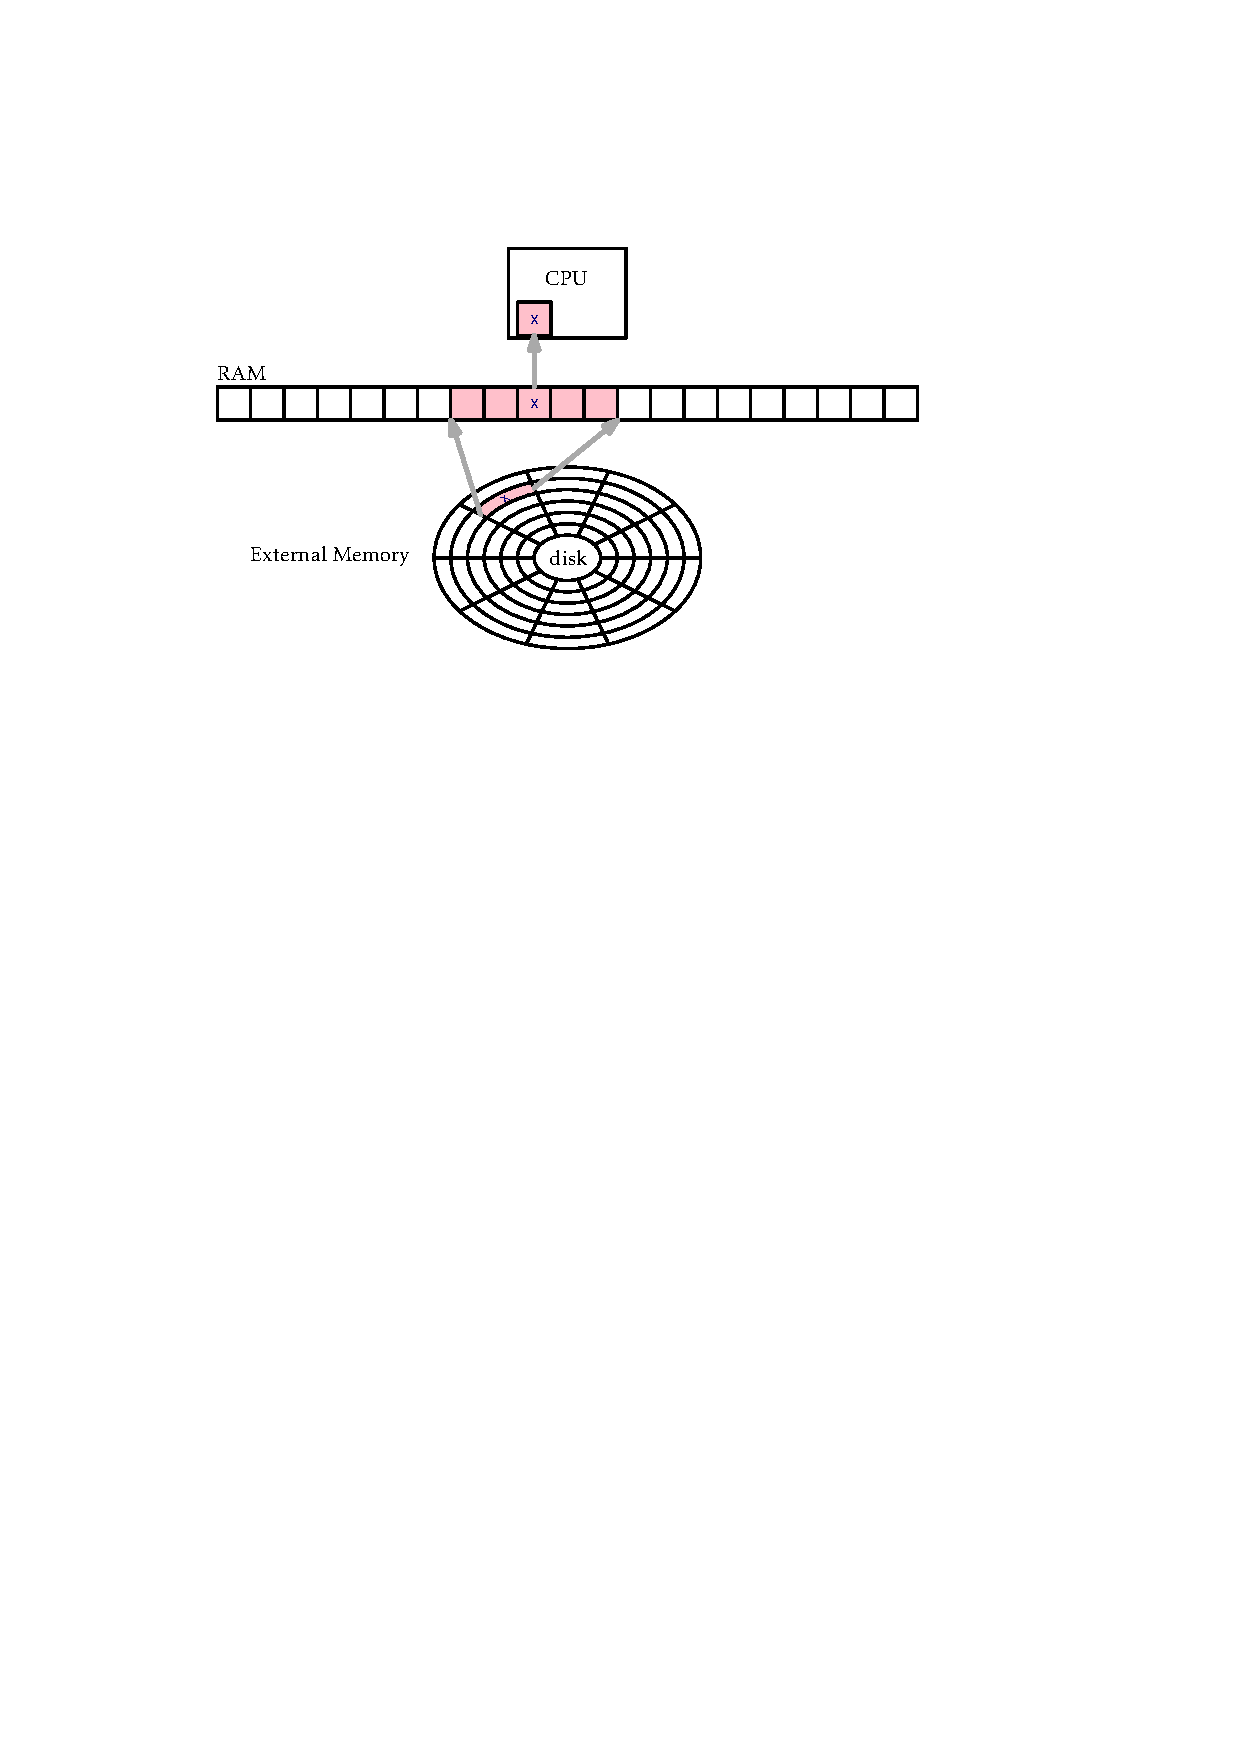
\includegraphics[width=\ScaleIfNeeded]{figs/em}}
  \caption[The external memory model]{In the external memory model,
  accessing an individual item, #x#, in the external memory requires
  reading the entire block containing #x# into RAM.}
  \figlabel{em}
\end{figure}

In the full-blown external memory model, the size of the internal
memory is also a parameter.  However, for the data structures described
in this chapter, it is sufficient to have an internal memory of size
$O(B+\log_B #n#)$.  That is, the memory needs to be capable of storing
a constant number of blocks and a recursion stack of height $O(\log_B
#n#)$.  In most cases, the $O(B)$ term dominates the memory requirement.
For example, even with the relatively small value $B=32$, $B\ge \log_B
#n#$ for all $#n#\le 2^{160}$.  In decimal, $B\ge \log_B #n#$ for any
\[
#n# \le 1\,461\,501\,637\,330\,902\,918\,203\,684\,832\,716\,283\,019\,655\,932\,542\,976 \enspace 
. \]

\section{The Block Store}

\index{block store}%
\index{BlockStore@#BlockStore#}%
The notion of external memory includes a large number of possible
different devices, each of which has its own block size and is
accessed with its own collection of system calls.  To simplify the
exposition of this chapter so that we can focus on the common ideas, we
encapsulate external memory devices with an object called a #BlockStore#.
A #BlockStore# stores a collection of memory blocks, each of size $B$.
Each block is uniquely identified by its integer index.  A #BlockStore#
supports these operations:

\begin{enumerate}
  \item #readBlock(i)#: Return the contents of the block whose index is #i#.

  \item #writeBlock(i,b)#: Write contents of #b# to the block whose
    index is #i#.

  \item #placeBlock(b)#: Return a new index and store the contents of #b#
    at this index.

  \item #freeBlock(i)#: Free the block whose index is #i#.  This indicates
    that the contents of this block are no longer used so the external
    memory allocated by this block may be reused.
\end{enumerate}

The easiest way to imagine a #BlockStore# is to imagine it as storing a
file on disk that is partitioned into blocks, each containing $B$ bytes.
In this way, #readBlock(i)# and #writeBlock(i,b)# simply read and write
bytes $#i#B,\ldots,(#i#+1)B-1$ of this file.  In addition, a simple
#BlockStore# could keep a \emph{free list} of blocks that are available
for use. Blocks freed with #freeBlock(i)# are added to the free list.
In this way, #placeBlock(b)# can use a block from the free list or,
if none is available, append a new block to the end of the file.


\section{B-Trees}
\seclabel{btree}

In this section, we discuss a generalization of binary trees,
called $B$-trees, which is efficient in the external memory model.
Alternatively, $B$-trees can be viewed as the natural generalization of
2-4 trees described in \secref{twofour}. (A 2-4 tree is a special case
of a $B$-tree that we get by setting $B=2$.)

\index{B-tree@$B$-tree}%
For any integer $B\ge 2$, a \emph{$B$-tree} is a tree in which all of
the leaves have the same depth and every non-root internal node, #u#,
has at least $B$ children and at most $2B$ children.  The children of #u#
are stored in an array, #u.children#.  The required number of children is
relaxed at the root, which can have anywhere between 2 and $2B$ children.

If the height of a $B$-tree is $h$, then it follows that the number,
$\ell$, of leaves in the $B$-tree satisfies
\[
    2B^{h-1} \le \ell \le 2(2B)^{h-1} \enspace .
\]
Taking the logarithm of the first inequality and rearranging terms yields:
\begin{align*}
    h & \le \frac{\log \ell-1}{\log B} + 1  \\
      & \le \frac{\log \ell}{\log B} + 1 \\
      & = \log_B \ell + 1 \enspace .
\end{align*}
That is, the height of a $B$-tree is proportional to the base-$B$
logarithm of the number of leaves.

Each node, #u#, in $B$-tree stores an array of keys
$#u.keys#[0],\ldots,#u.keys#[2B-1]$.  If #u# is an internal node with $k$
children, then the number of keys stored at #u# is exactly $k-1$ and these
are stored in $#u.keys#[0],\ldots,#u.keys#[k-2]$.  The remaining $2B-k+1$
array entries in #u.keys# are set to #null#.  If #u# is a non-root leaf
node, then #u# contains between $B-1$ and $2B-1$ keys. The keys in a
$B$-tree respect an order similar to the keys in a binary search tree.
For any node, #u#, that stores $k-1$ keys,
\[
   #u.keys[0]# < #u.keys[1]# < \cdots < #u.keys#[k-2] \enspace .
\]
If #u# is an internal node, then for every $#i#\in\{0,\ldots,k-2\}$,
$#u.keys[i]#$ is larger than every key stored in the subtree rooted at
#u.children[i]# but smaller than every key stored in the subtree rooted
at $#u.children[i+1]#$.  Informally,
\[
   #u.children[i]# \prec #u.keys[i]# \prec #u.children[i+1]# \enspace .
\]
An example of a $B$-tree with $B=2$ is shown in \figref{btree}.

\begin{figure}
  \centering{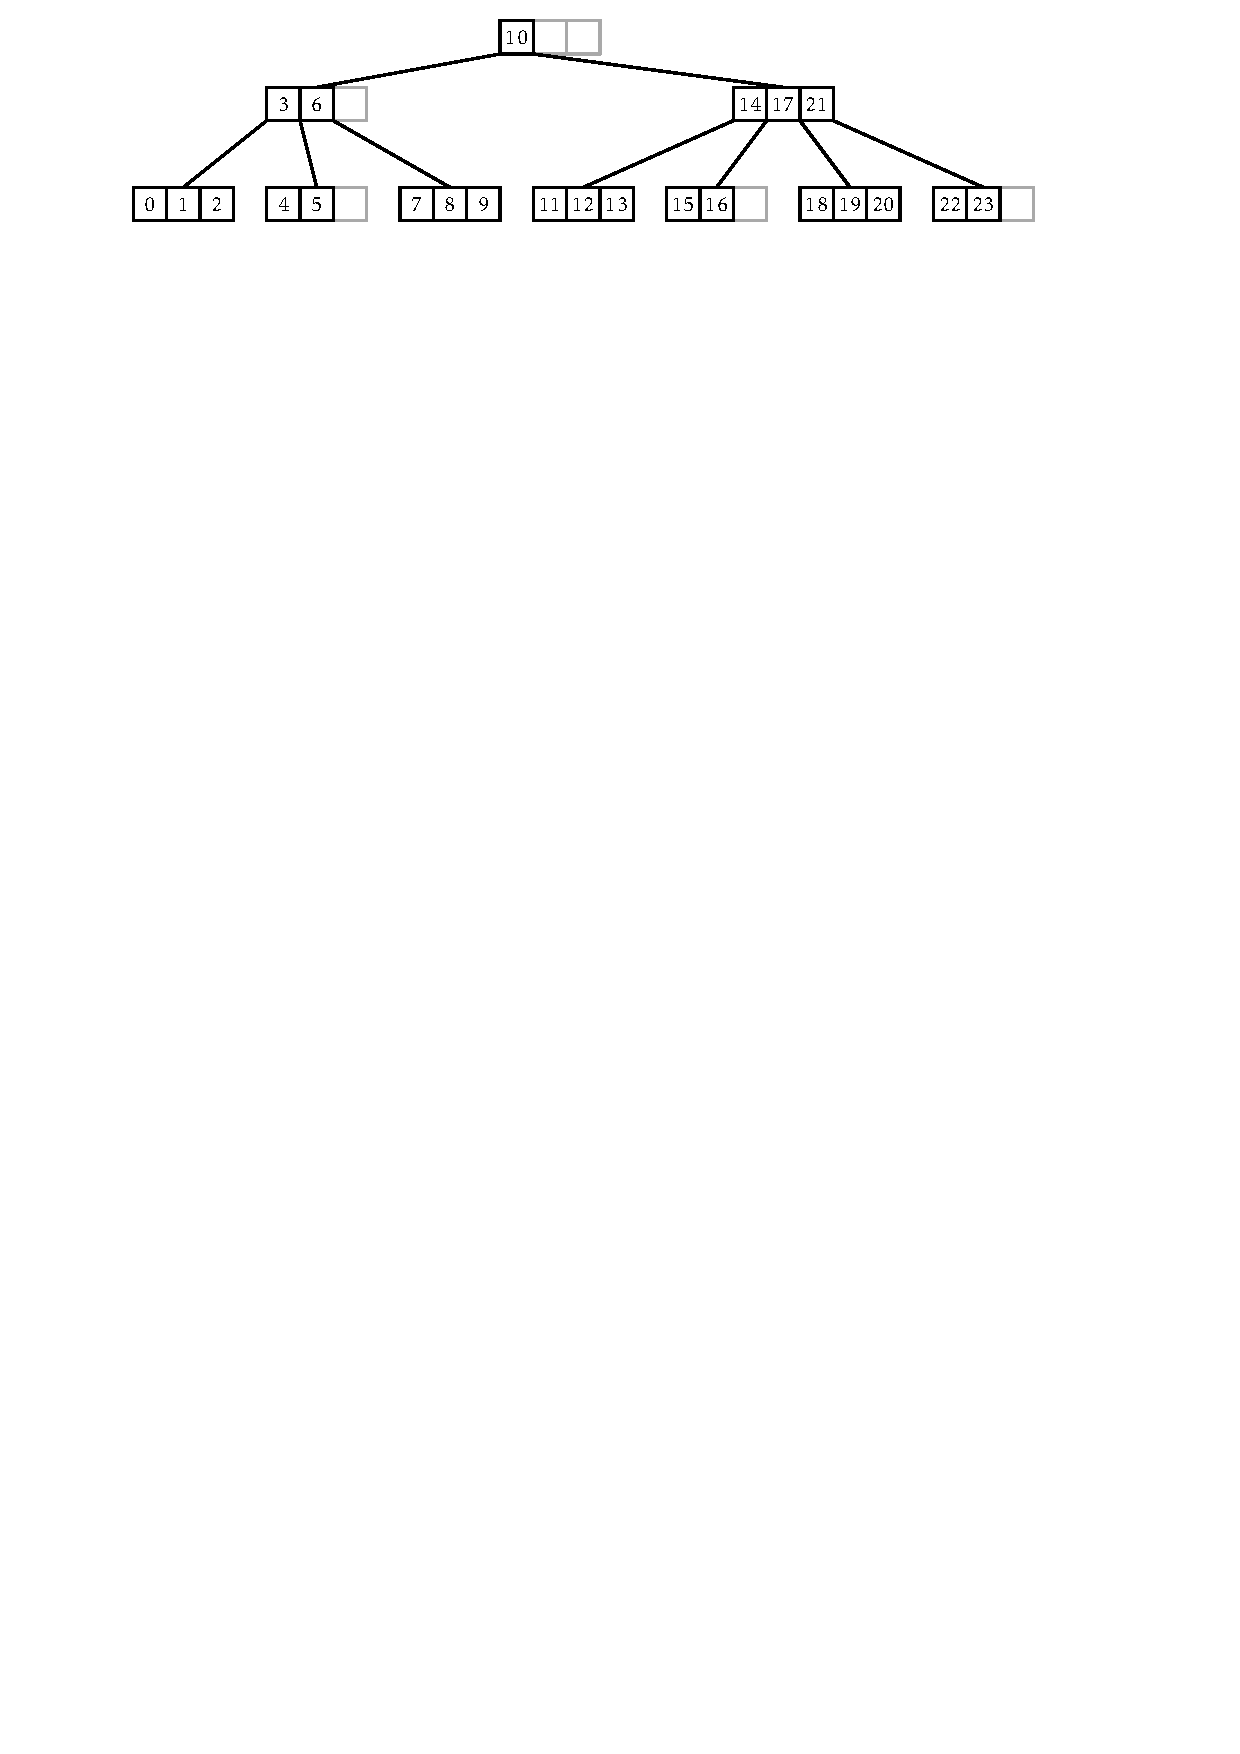
\includegraphics[width=\ScaleIfNeeded]{figs/btree-1}}
  \caption{A $B$-tree with $B=2$.}
  \figlabel{btree}
\end{figure}

Note that the data stored in a $B$-tree node has size $O(B)$.  Therefore,
in an external memory setting, the value of $B$ in a $B$-tree is chosen
so that  a node fits into a single external memory block.  In this way,
the time it takes to perform a $B$-tree operation in the external memory
model is proportional to the number of nodes that are accessed (read or
written) by the operation.

For example, if the keys are 4 byte integers and the node indices are
also 4 bytes, then setting $B=256$ means that each node stores
\[
(4+4)\times 2B
 = 8\times512=4096
\]
bytes of data.  This would be a perfect value of $B$ for the hard disk
or solid state drive discussed in the introduction to this chaper,
which have a block size of $4096$ bytes.

The #BTree# class, which implements a $B$-tree, stores a #BlockStore#,
#bs#, that stores #BTree# nodes as well as the index, #ri#, of the
root node.  As usual, an integer, #n#, is used to keep track of the number
of items in the data structure:
\cppimport{ods/BTree.n.ri.bs}
\javaimport{ods/BTree.n.ri.bs}
\pcodeimport{ods/BTree.initialize(b)}

\subsection{Searching}

The implementation of the #find(x)# operation, which is illustrated in
\figref{btree-find}, generalizes the #find(x)# operation in a binary
search tree.  The search for #x# starts at the root and uses the keys
stored at a node, #u#, to determine in which of #u#'s children the search
should continue.

\begin{figure}
  \centering{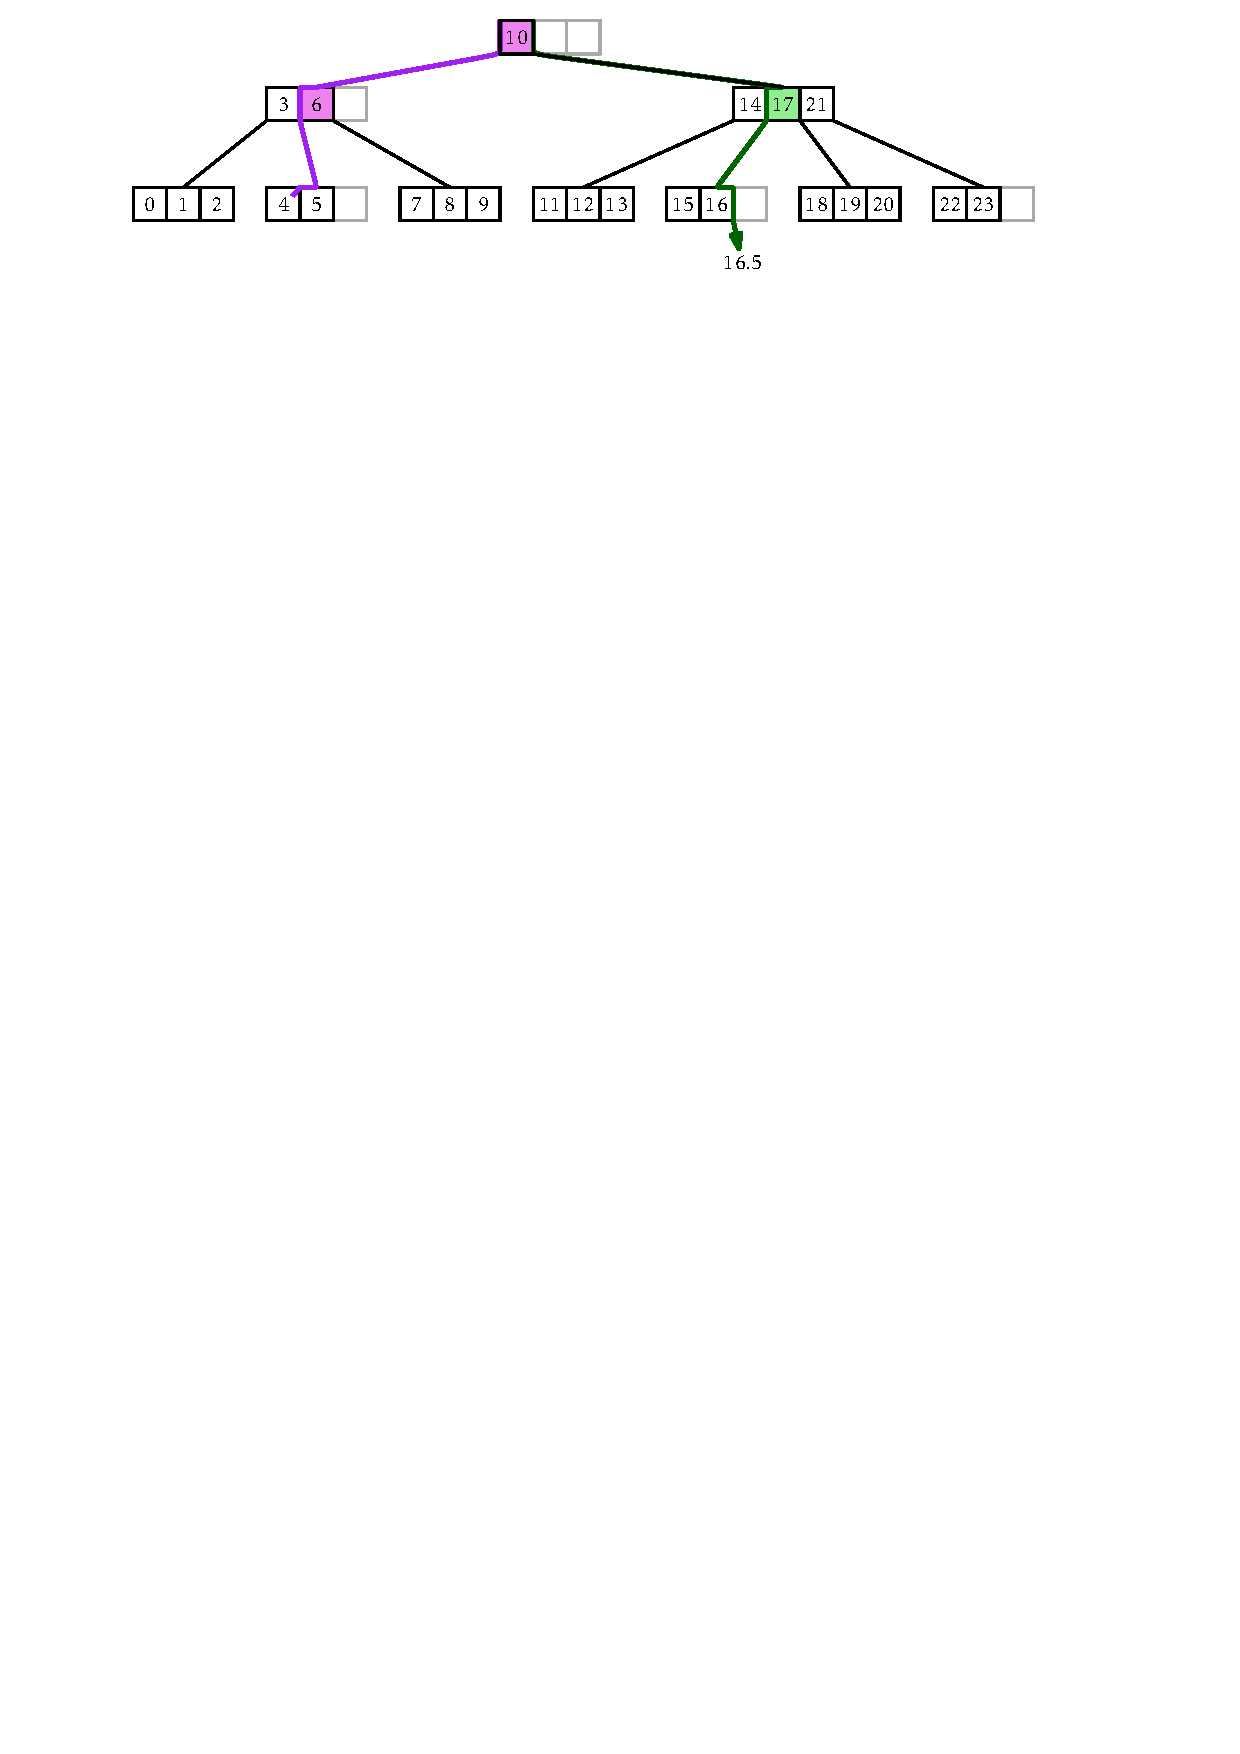
\includegraphics[width=\ScaleIfNeeded]{figs/btree-2}}
  \caption[Searching in a $B$-tree]{A successful search (for the value 4)
    and an unsuccessful search (for the value 16.5) in a $B$-tree. Shaded nodes show where the value of #z# is updated during the searches.}
  \figlabel{btree-find}
\end{figure}
More specifically, at a node #u#, the search checks if #x# is stored
in #u.keys#.  If so, #x# has been found and the search is complete.
Otherwise, the search finds the smallest integer, #i#, such that
$#u.keys[i]# > #x#$ and continues the search in the subtree rooted at
#u.children[i]#.  If no key in #u.keys# is greater than #x#, then the
search continues in #u#'s rightmost child.  Just like binary search
trees, the algorithm keeps track of the most recently seen key, #z#,
that is larger than #x#.  In case #x# is not found, #z# is returned as
the smallest value that is greater or equal to #x#.
\codeimport{ods/BTree.find(x)}
Central to the #find(x)# method is the #findIt(a,x)# method that
searches in a #null#-padded sorted array, #a#, for the value #x#.
This method, illustrated in \figref{findit}, works for any array,
#a#, where $#a#[0],\ldots,#a#[k-1]$ is a sequence of keys in sorted
order and $#a#[k],\ldots,#a#[#a.length#-1]$ are all set to #null#.
If #x# is in the array at position #i#, then #findIt(a,x)# returns
$-#i#-1$. Otherwise, it returns the smallest index, #i#, such that
$#a[i]#>#x#$ or $#a[i]#=#null#$.
\begin{figure}
  \centering{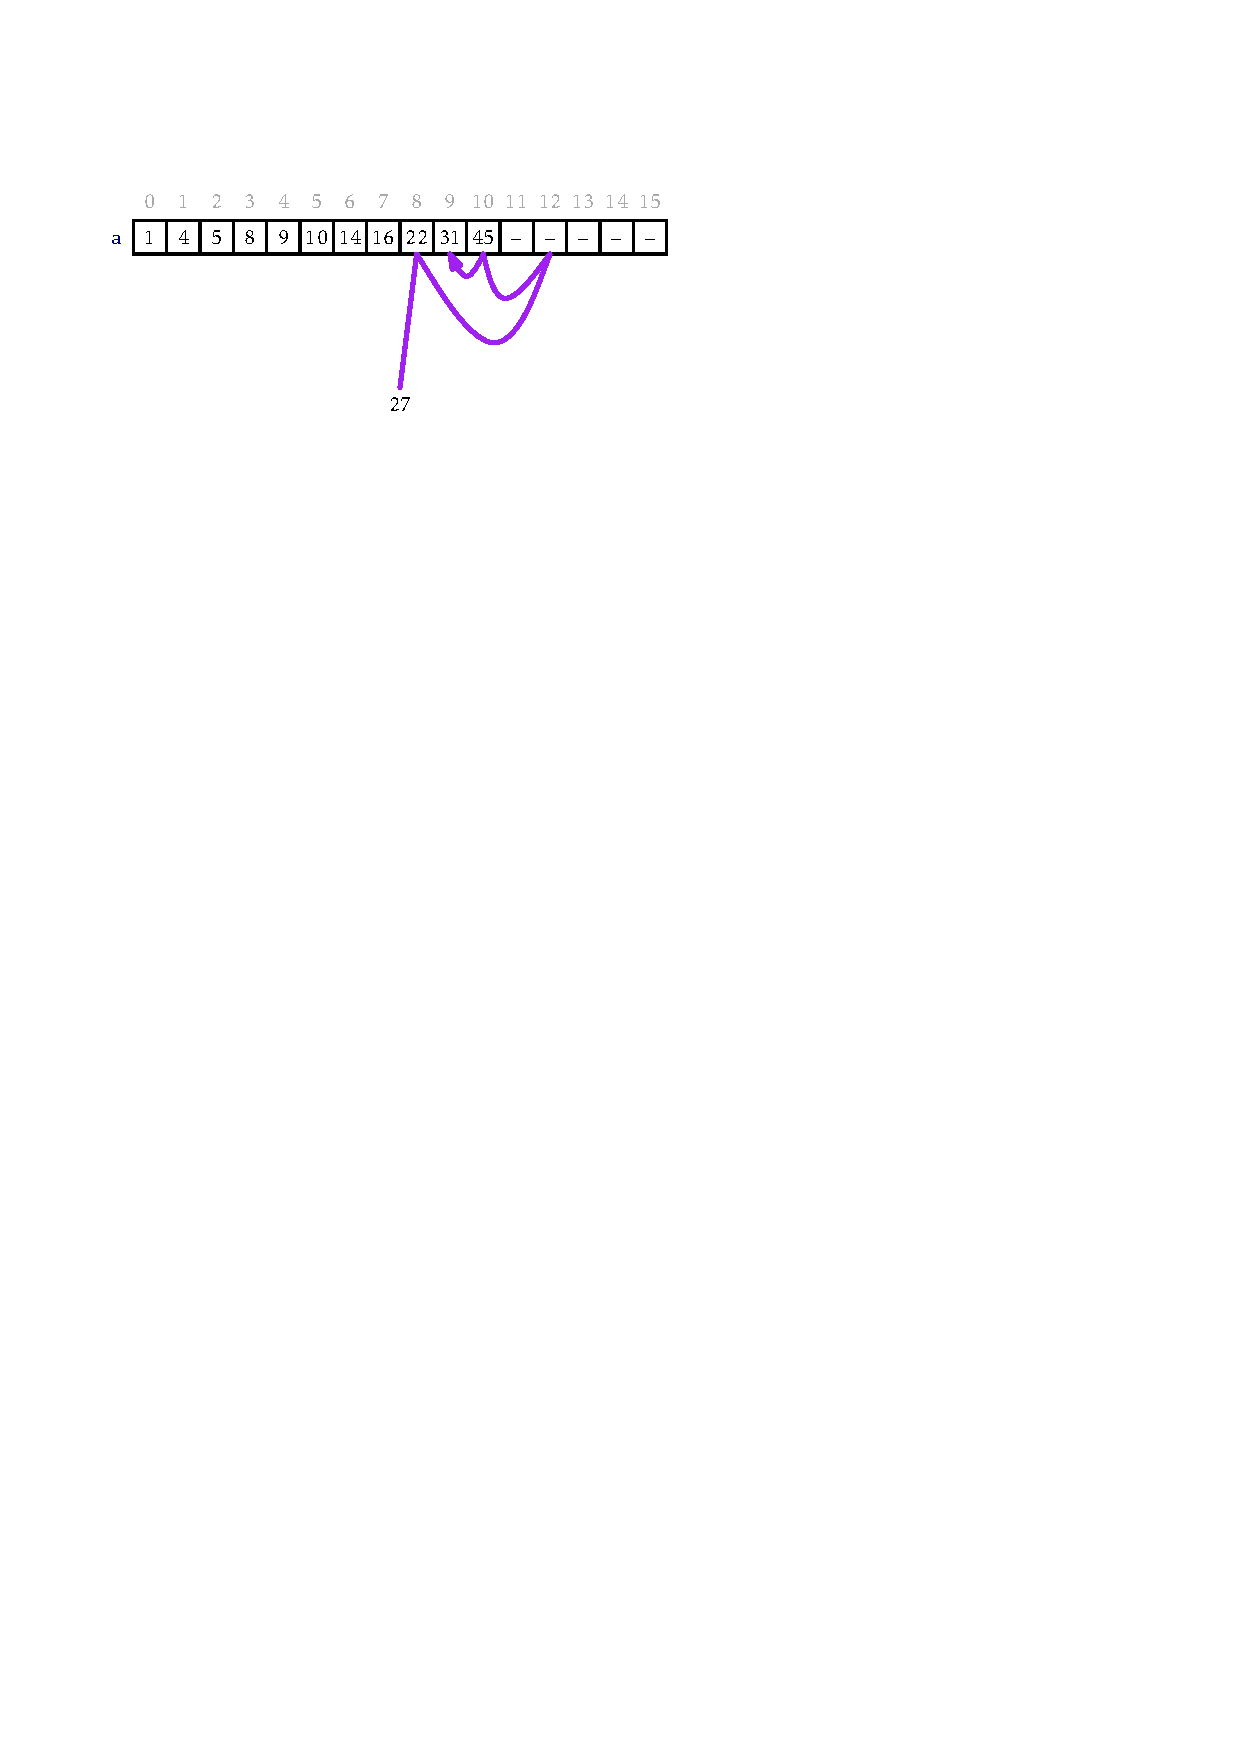
\includegraphics[scale=0.90909]{figs/findit}}
  \caption[The findIt(a,x) method]{The execution of #findIt(a,27)#.}
  \figlabel{findit}
\end{figure}
\codeimport{ods/BTree.findIt(a,x)}
The #findIt(a,x)# method uses a binary search 
\index{binary search}%
that halves the search
space at each step, so it runs in $O(\log(#a.length#))$ time.  In our setting, $#a.length#=2B$, so #findIt(a,x)# runs in $O(\log B)$ time.

We can analyze the running time of a $B$-tree #find(x)# operation both
in the usual word-RAM model (where every instruction counts) and in the
external memory model (where we only count the number of nodes accessed).
Since each leaf in a $B$-tree stores at least one key and the height
of a $B$-Tree with $\ell$ leaves is $O(\log_B\ell)$, the height of a
$B$-tree that stores #n# keys is $O(\log_B #n#)$.  Therefore, in the
external memory model, the time taken by the #find(x)# operation is
$O(\log_B #n#)$.  To determine the running time in the word-RAM model,
we have to account for the cost of calling #findIt(a,x)# for each node
we access, so the running time of #find(x)# in the word-RAM model is
\[
   O(\log_B #n#)\times O(\log B) = O(\log #n#) \enspace .
\]

\subsection{Addition}

One important difference between $B$-trees and the #BinarySearchTree#
data structure from \secref{binarysearchtree} is that the nodes of a
$B$-tree do not store pointers to their parents.  The reason for this
will be explained shortly.  The lack of parent pointers means that
the #add(x)# and #remove(x)# operations on $B$-trees are most easily
implemented using recursion.

Like all balanced search trees, some form of rebalancing is required
during an #add(x)# operation.  In a $B$-tree, this is done by
\emph{splitting} nodes.
\index{split}%
Refer to \figref{btree-split} for what follows.
Although splitting takes place across two levels of recursion, it is
best understood as an operation that takes a node #u# containing $2B$
keys and having $2B+1$ children.  It creates a new node, #w#, that
adopts $#u.children#[B],\ldots,#u.children#[2B]$.  The new node #w#
also takes #u#'s $B$ largest keys, $#u.keys#[B],\ldots,#u.keys#[2B-1]$.
At this point, #u# has $B$ children and $B$ keys.  The extra key,
$#u.keys#[B-1]$, is passed up to the parent of #u#, which also adopts #w#.

Notice that the splitting operation modifies three nodes: #u#, #u#'s
parent, and the new node, #w#.   This is why it is important that the
nodes of a $B$-tree do not maintain parent pointers.  If they did, then
the $B+1$ children adopted by #w# would all need to have their parent
pointers modified. This would increase the number of external memory
accesses from 3 to $B+4$ and would make $B$-trees much less efficient for
large values of $B$.

\begin{figure}
   \centering{\begin{tabular}{@{}l@{}}
     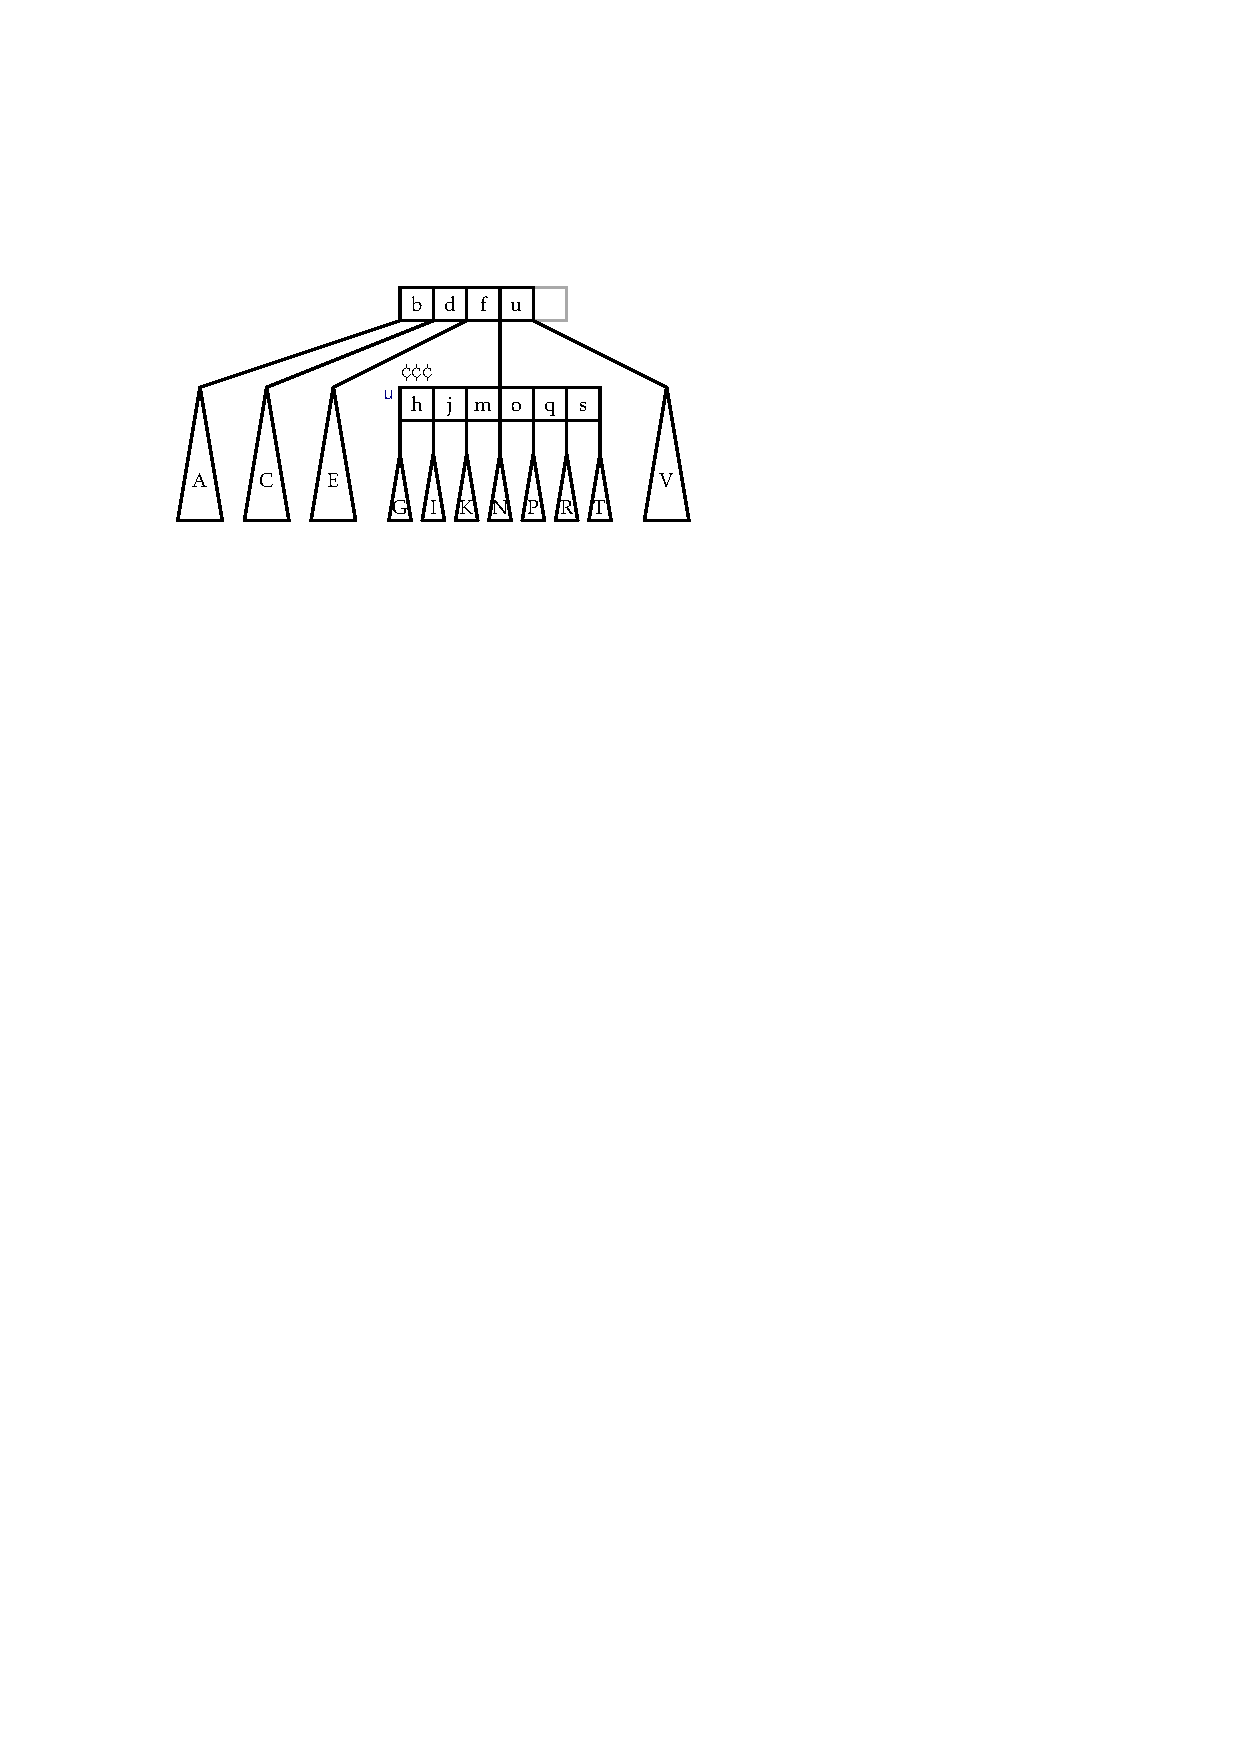
\includegraphics[width=\ScaleIfNeeded]{figs/btree-split-1} \\[2ex]
     \multicolumn{1}{c}{#u.split()#} \\ 
     \multicolumn{1}{c}{$\Downarrow$} \\[2ex]
     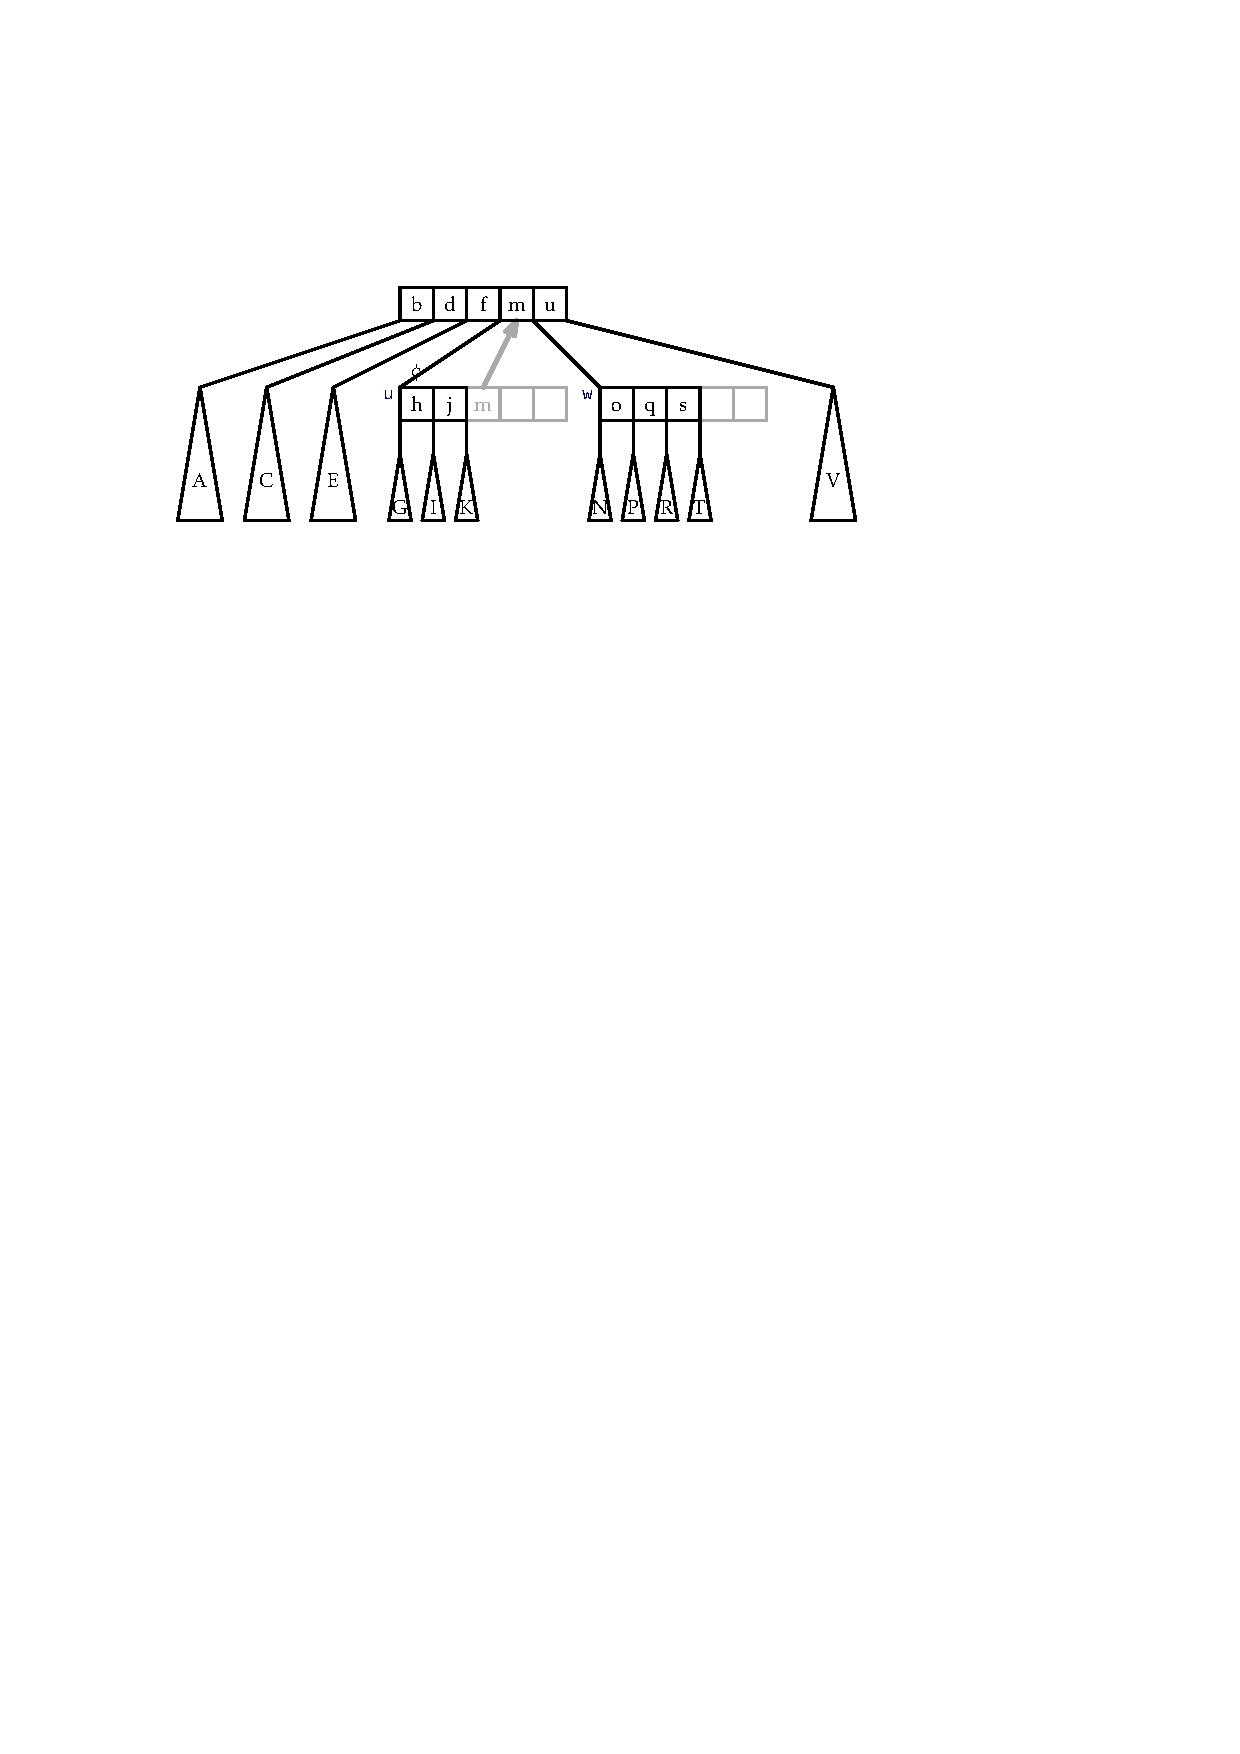
\includegraphics[width=\ScaleIfNeeded]{figs/btree-split-2} \\
   \end{tabular}}
   \caption[Splitting a $B$-tree node]{Splitting the node #u# in a
     $B$-tree ($B=3$). Notice that the key $#u.keys#[2]=\mathrm{m}$
     passes from #u# to its parent.}
   \figlabel{btree-split}
\end{figure}

The #add(x)# method in a $B$-tree is illustrated in \figref{btree-add}.
At a high level, this method finds a leaf, #u#, at which to add the
value #x#.  If this causes #u# to become overfull (because it already
contained $B-1$ keys), then #u# is split.  If this causes #u#'s parent to
become overfull, then #u#'s parent is also split, which may cause #u#'s
grandparent to become overfull, and so on. This process continues,
moving up the tree one level at a time until reaching a node that
is not overfull or until the root is split. In the former case, the
process stops.  In the latter case, a new root is created whose two
children become the nodes obtained when the original root was split.

\begin{figure}
   \centering{\begin{tabular}{@{}l@{}}
     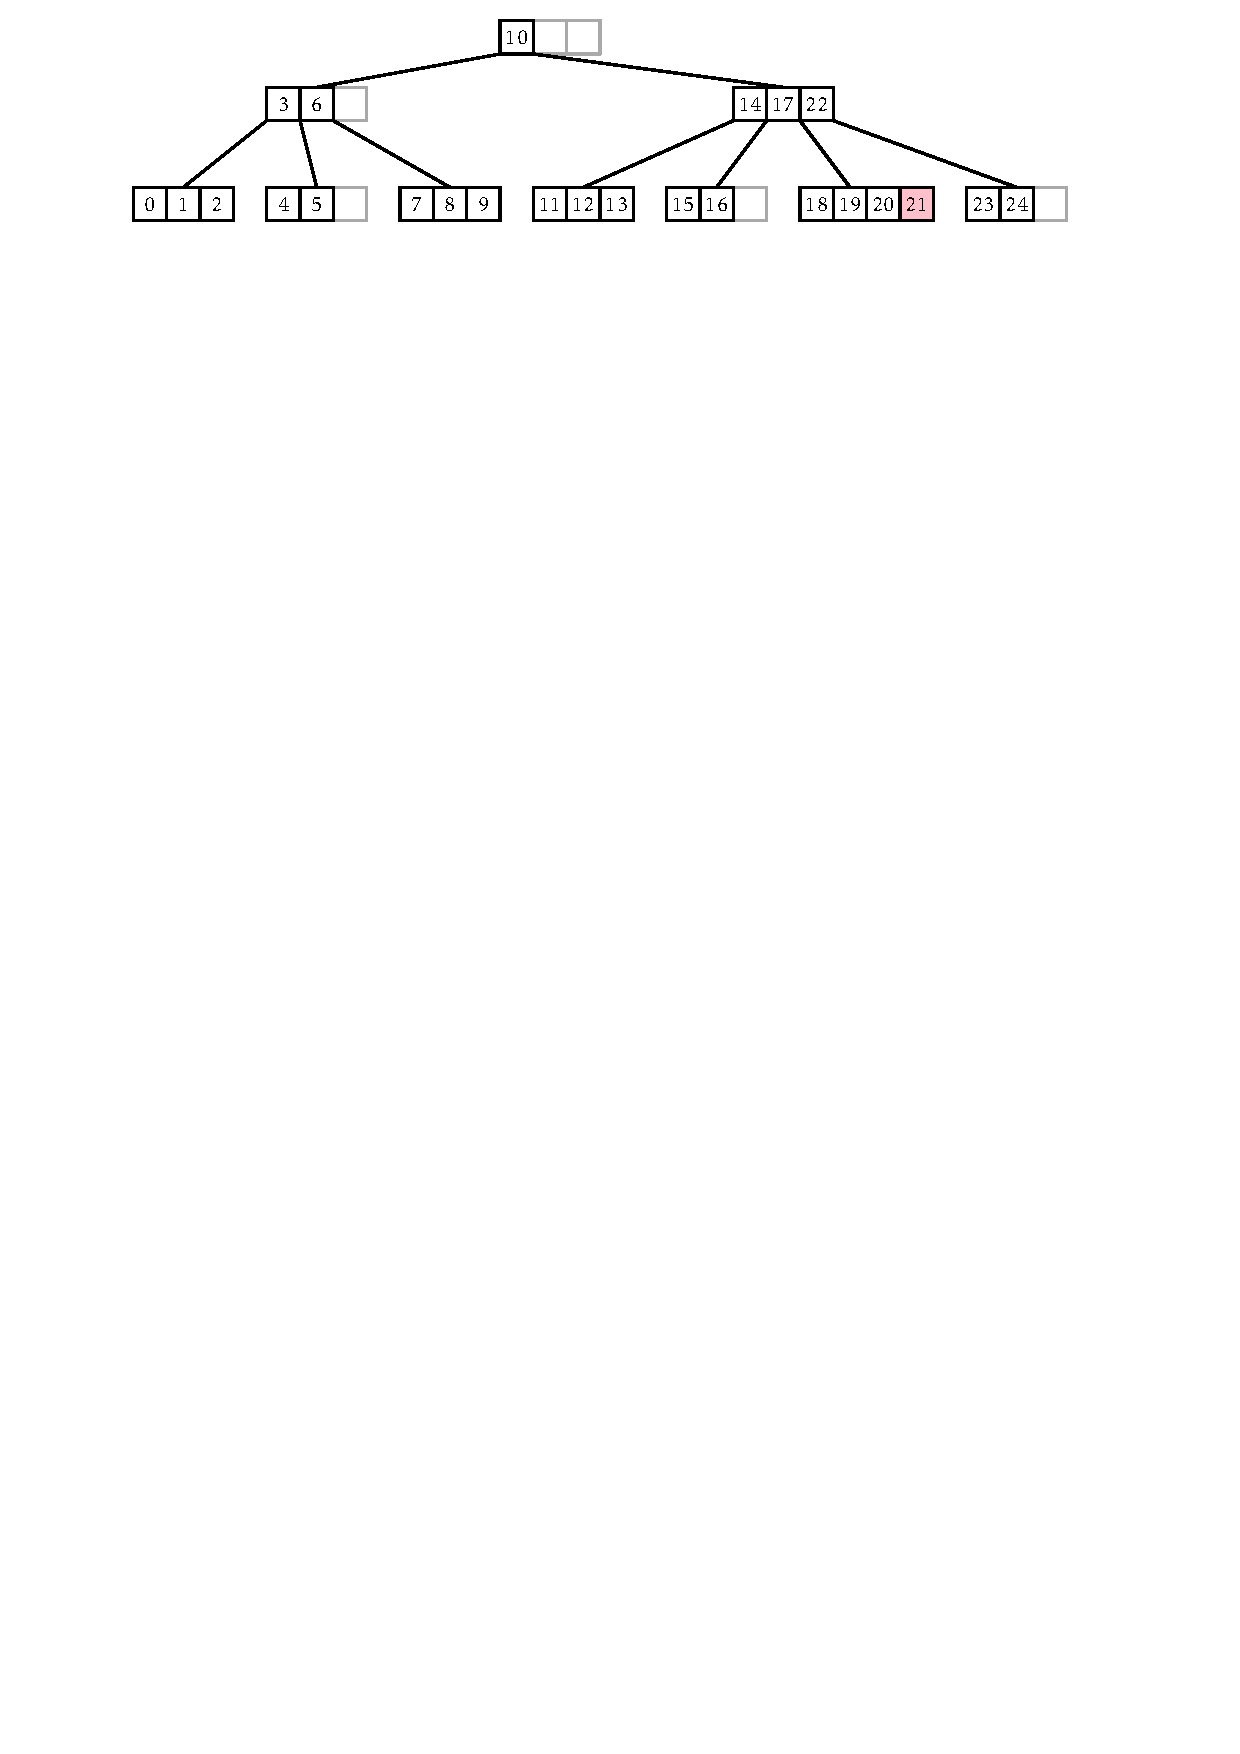
\includegraphics[width=\ScaleIfNeeded]{figs/btree-add-1} \\[2ex]
     \multicolumn{1}{c}{$\Downarrow$} \\[2ex]
     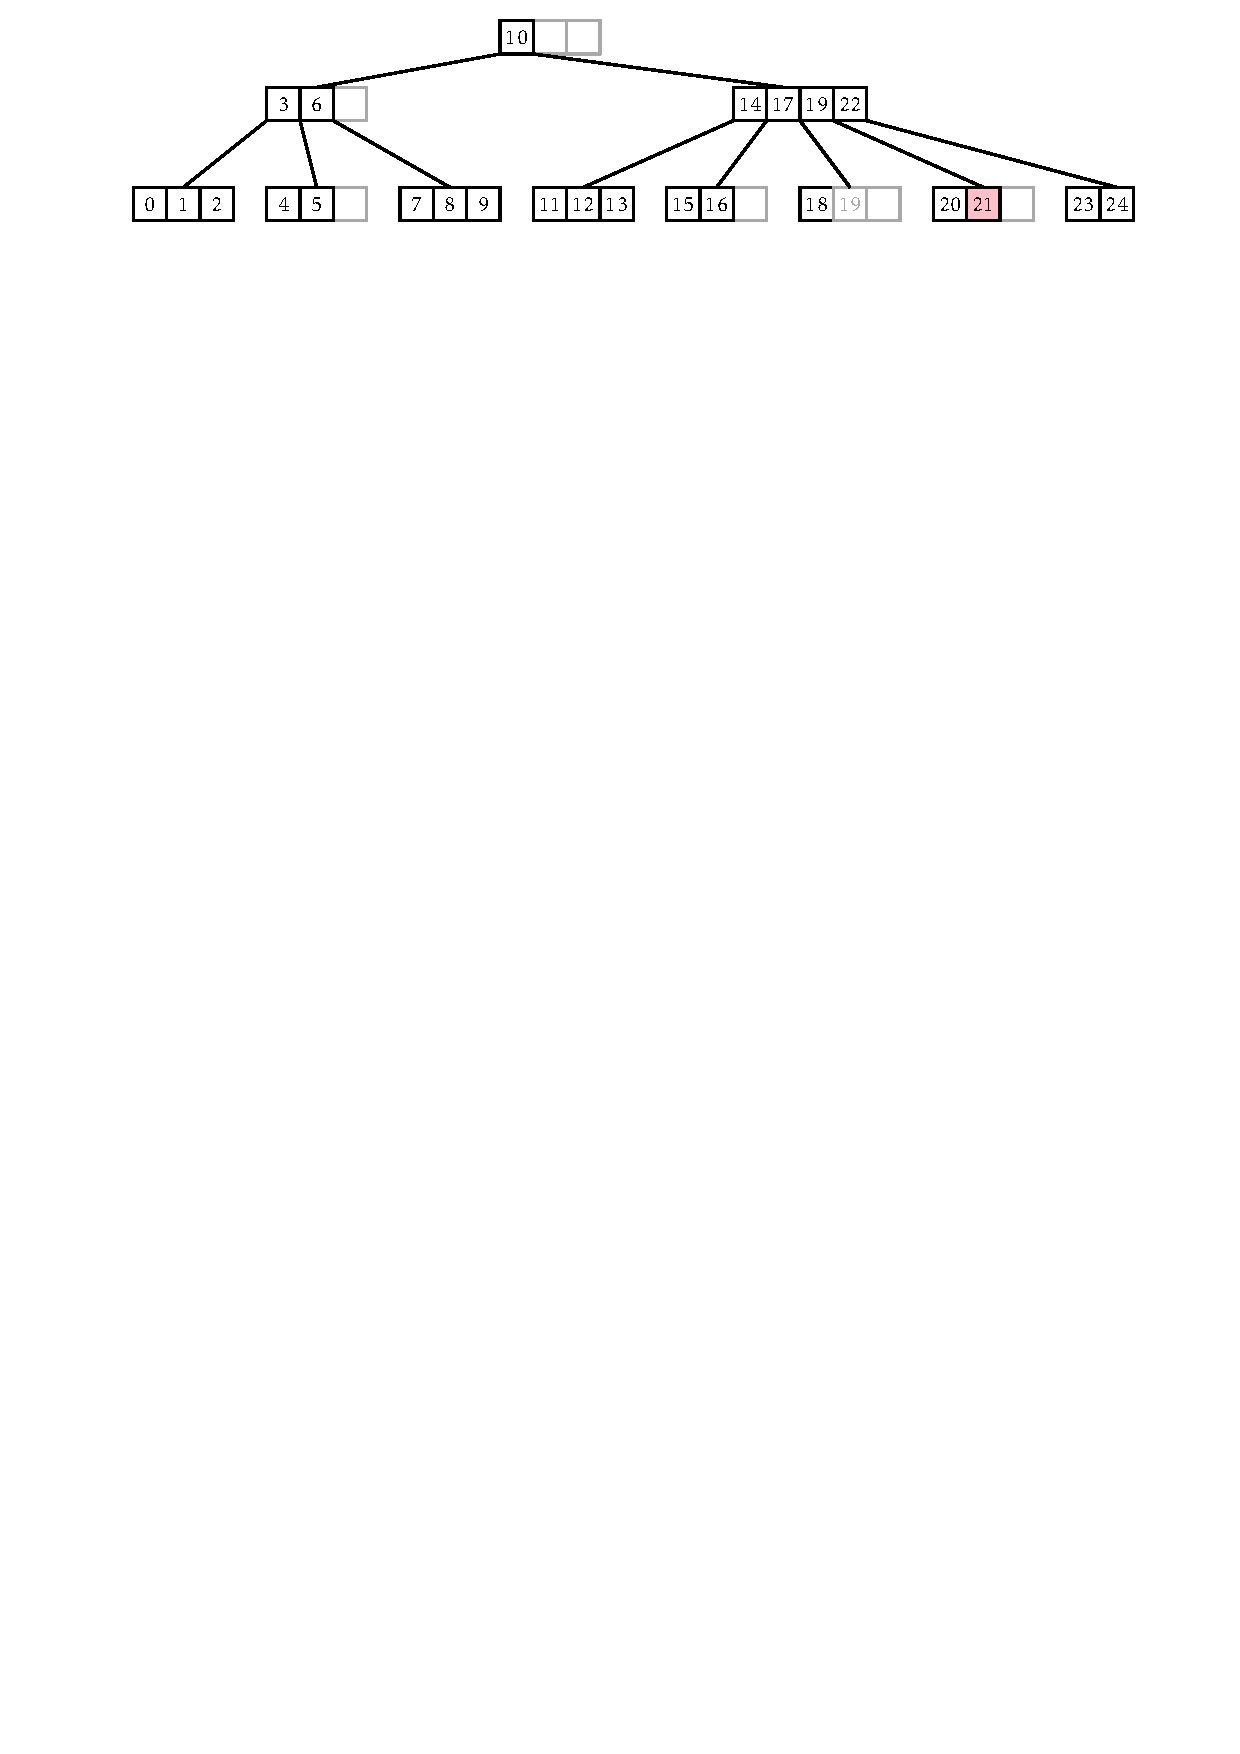
\includegraphics[width=\ScaleIfNeeded]{figs/btree-add-2} \\[2ex]
     \multicolumn{1}{c}{$\Downarrow$} \\[2ex]
     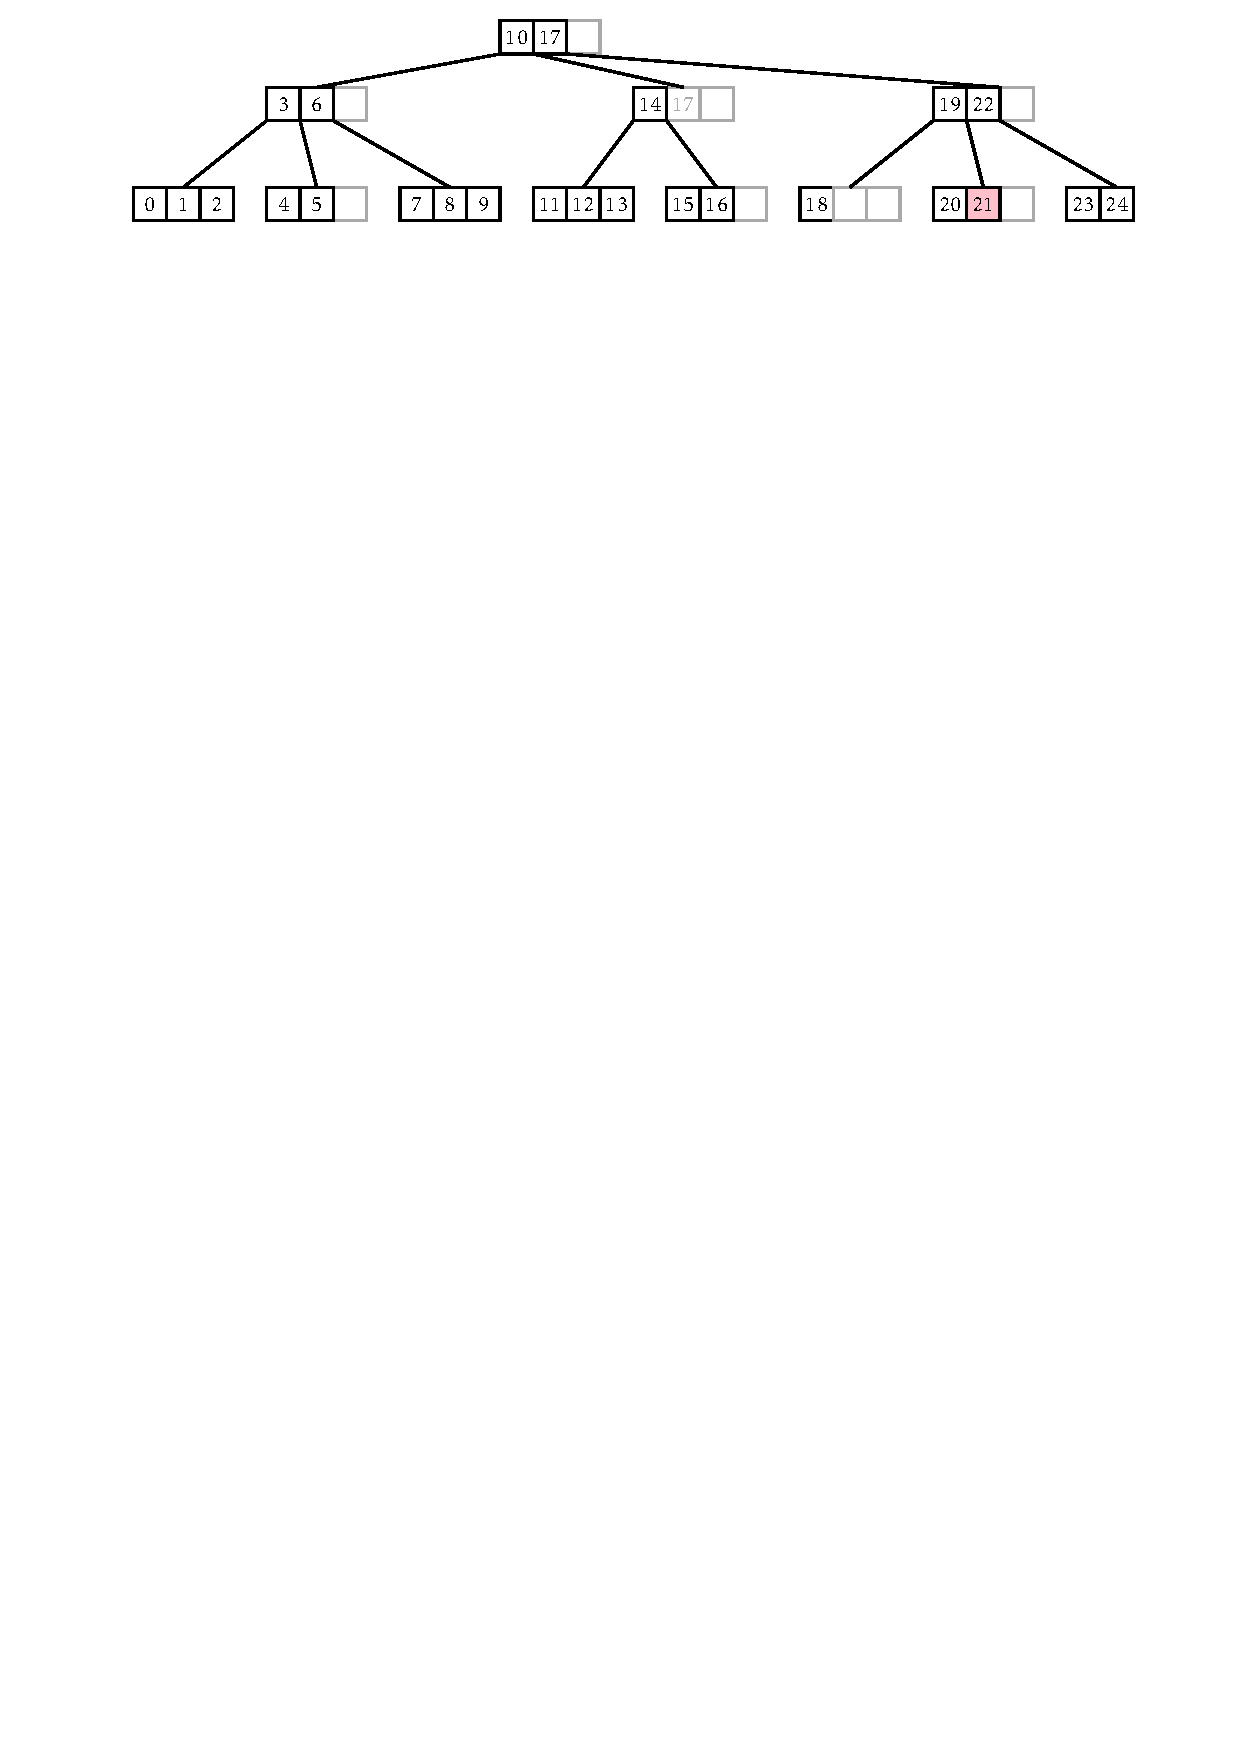
\includegraphics[width=\ScaleIfNeeded]{figs/btree-add-3} 
   \end{tabular}}
   \caption[Adding to a $B$-tree]{The #add(x)# operation in a
      #BTree#. Adding the value 21 results in two nodes being split.}
   \figlabel{btree-add}
\end{figure}

The executive summary of the #add(x)# method is that it walks
from the root to a leaf searching for #x#, adds #x# to this leaf, and
then walks back up to the root, splitting any overfull nodes it encounters
along the way.  With this high level view in mind, we can now delve into
the details of how this method can be implemented recursively.

The real work of #add(x)# is done by the #addRecursive(x,ui)# method,
which adds the value #x# to the subtree whose root, #u#, has the
identifier #ui#.  If #u# is a leaf, then #x# is simply inserted into
#u.keys#.  Otherwise, #x# is added recursively into the appropriate
child, $#u#'$, of #u#.  The result of this recursive call is normally
#null# but may also be a reference to a newly-created node, #w#, that
was created because $#u#'$ was split.  In this case, #u# adopts #w#
and takes its first key, completing the splitting operation on $#u#'$.

After the value #x# has been added (either to #u# or to a descendant of #u#),
the #addRecursive(x,ui)# method checks to see if #u# is storing too many
(more than $2B-1$) keys.  If so, then #u# needs to be \emph{split}
with a call to the #u.split()# method.  The result of calling #u.split()#
is a new node that is used as the return value for #addRecursive(x,ui)#.
\codeimport{ods/BTree.addRecursive(x,ui)}

The #addRecursive(x,ui)# method is a helper for the #add(x)# method, which
calls #addRecursive(x,ri)# to insert #x# into the root of the $B$-tree.
If #addRecursive(x,ri)# causes the root to split, then a new root is
created that takes as its children both the old root and the new node
created by the splitting of the old root.
\codeimport{ods/BTree.add(x)}

The #add(x)# method and its helper, #addRecursive(x,ui)#, can be analyzed
in two phases:

\begin{description}
  \item[Downward phase:]
    During the downward phase of the recursion, before #x# has been added,
    they access a sequence of #BTree# nodes and call #findIt(a,x)# on each node.
    As with the #find(x)# method, this takes $O(\log_B #n#)$ time in the
    external memory model and $O(\log #n#)$ time in the word-RAM model.
  
  \item[Upward phase:]
    During the upward phase of the recursion, after #x# has been added,
    these methods perform a sequence of at most $O(\log_B #n#)$ splits.
    Each split involves only three nodes, so this phase takes $O(\log_B
    #n#)$ time in the external memory model.  However, each split
    involves moving $B$ keys and children from one node to another, so
    in the word-RAM model, this takes $O(B\log #n#)$ time.
\end{description}

Recall that the value of $B$ can be quite large, much larger
than even $\log #n#$.  Therefore, in the word-RAM model, adding a value
to a $B$-tree can be much slower than adding into a balanced binary
search tree.  Later, in \secref{btree-amortized}, we will show that the
situation is not quite so bad; the amortized number of split operations
done during an #add(x)# operation is constant.  This shows that the
(amortized) running time of the #add(x)# operation in the word-RAM model
is $O(B+\log #n#)$.


\subsection{Removal}

The #remove(x)# operation in a #BTree# is, again, most easily implemented
as a recursive method.  Although the recursive implementation of
#remove(x)# spreads the complexity across several methods, the overall
process, which is illustrated in \figref{btree-remove-full}, is fairly
straightforward.  By shuffling keys around, removal is reduced to the
problem of removing a value, $#x#'$, from some leaf, #u#.  Removing $#x#'$
may leave #u# with less than $B-1$  keys;  this situation is called
an \emph{underflow}.
\index{underflow}%

\begin{figure}
   \centering{\begin{tabular}{@{}l@{}}
     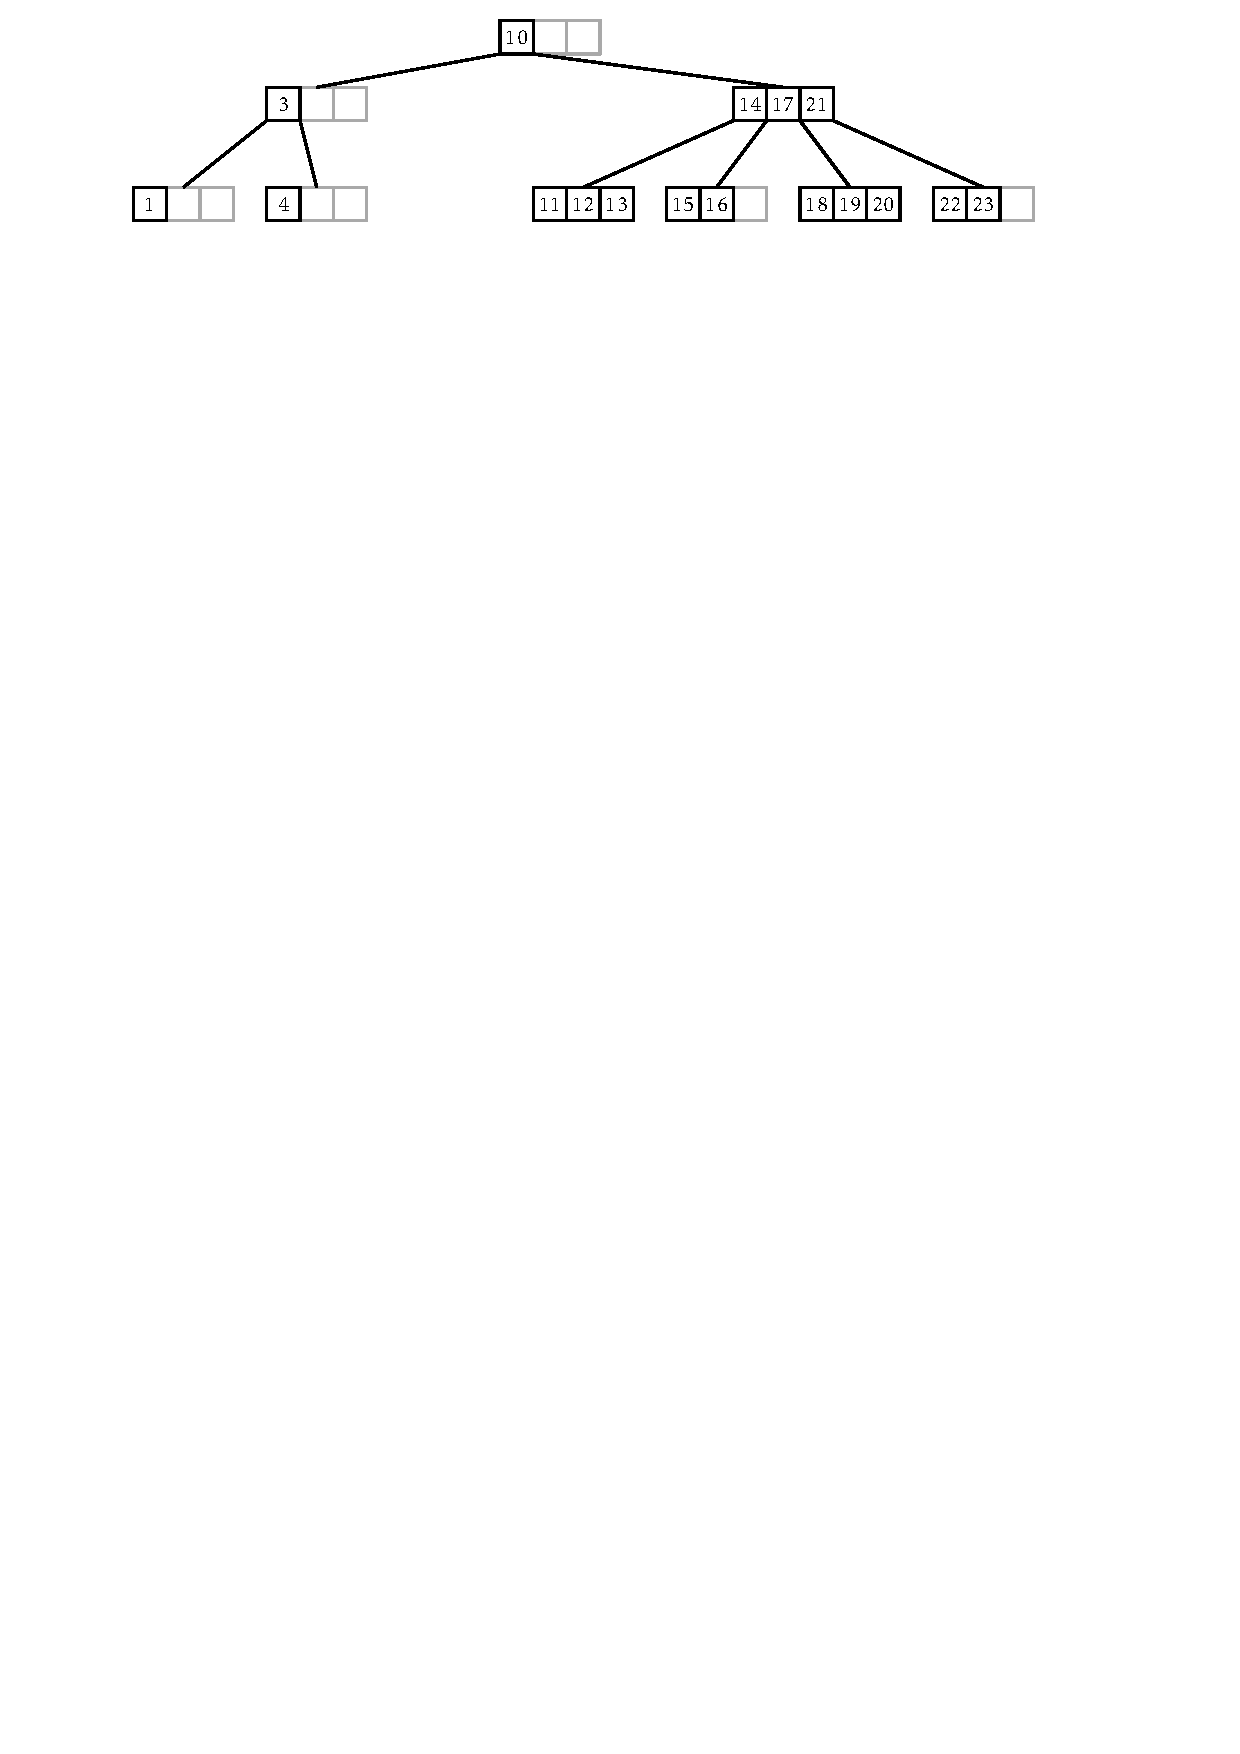
\includegraphics[width=\ScaleIfNeeded]{figs/btree-remove-full-1} \\[2ex]
     \multicolumn{1}{c}{$\Downarrow$} \\[2ex]
     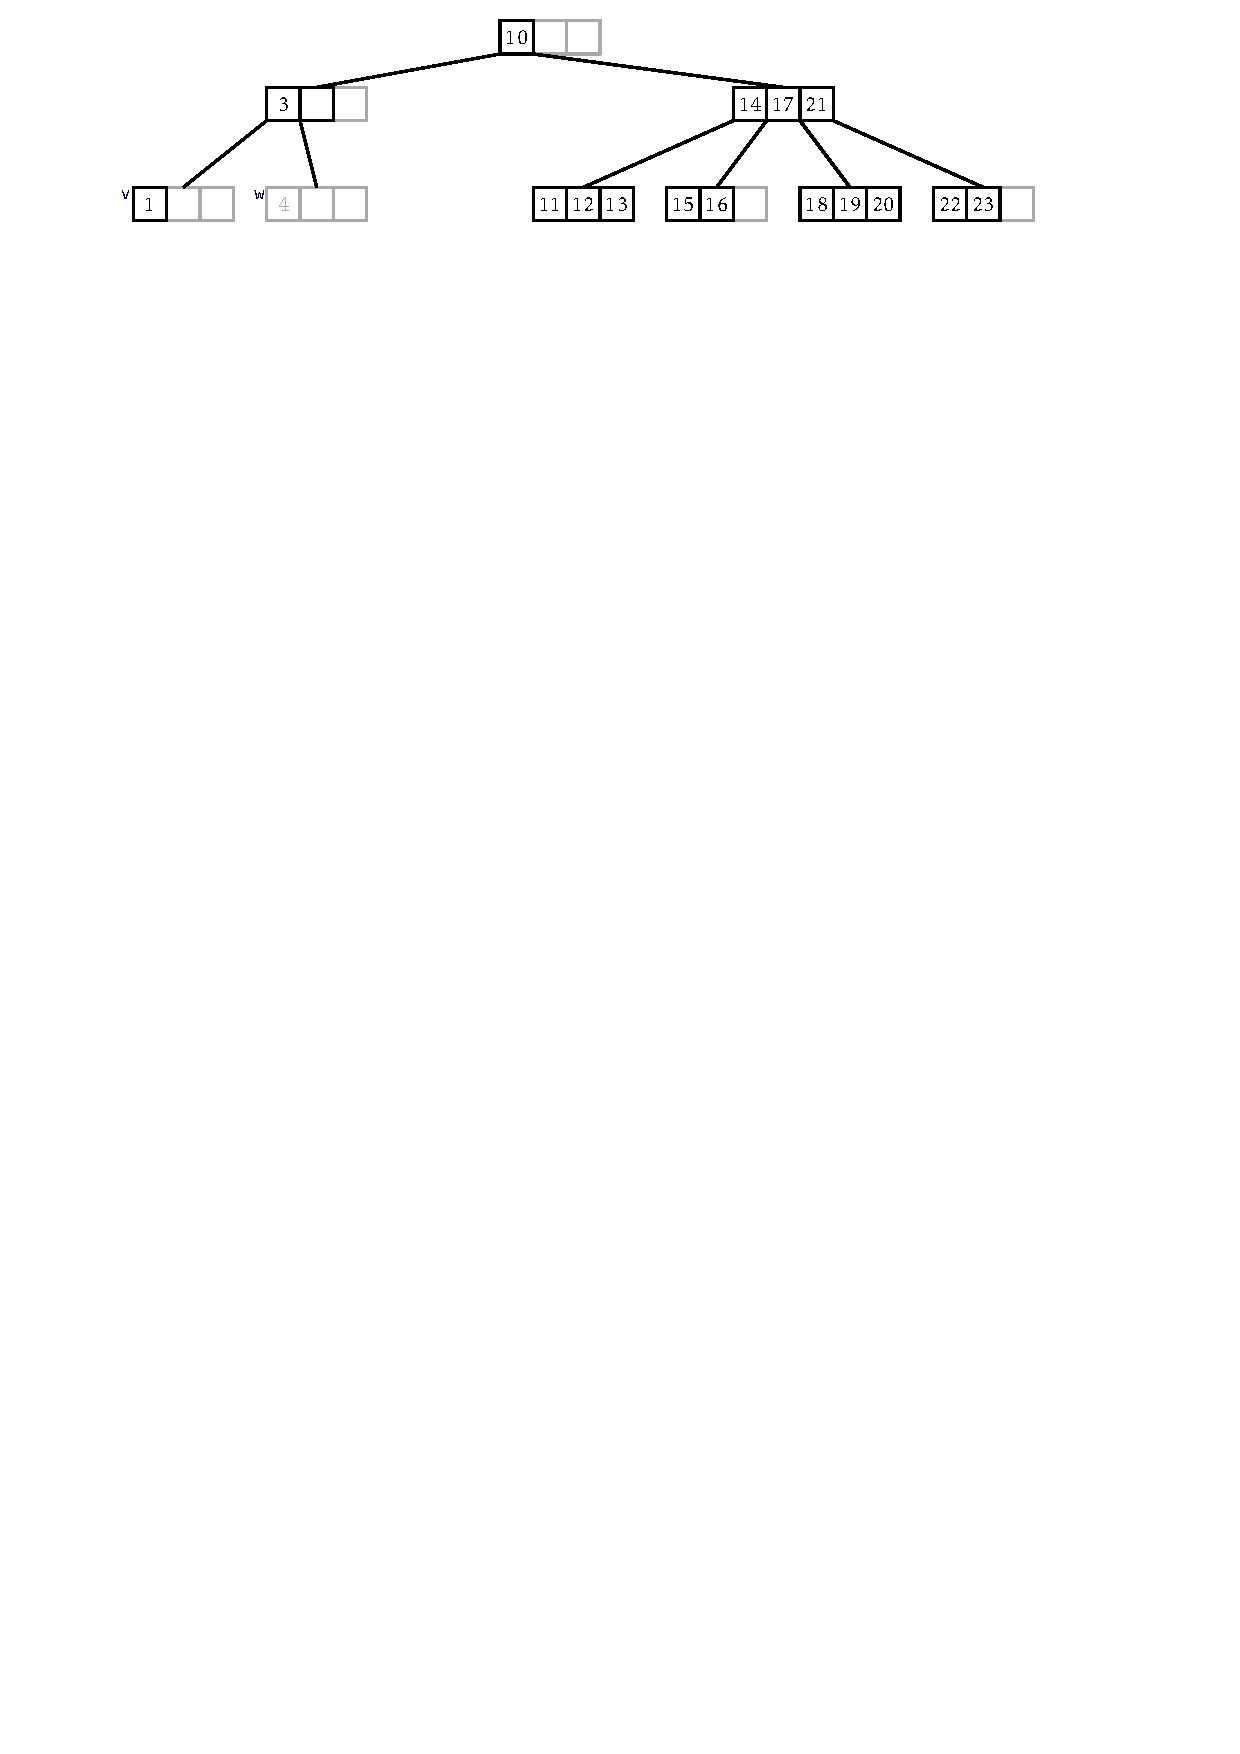
\includegraphics[width=\ScaleIfNeeded]{figs/btree-remove-full-2} \\[2ex]
     \multicolumn{1}{c}{#merge(v,w)#} \\
     \multicolumn{1}{c}{$\Downarrow$} \\[2ex]
     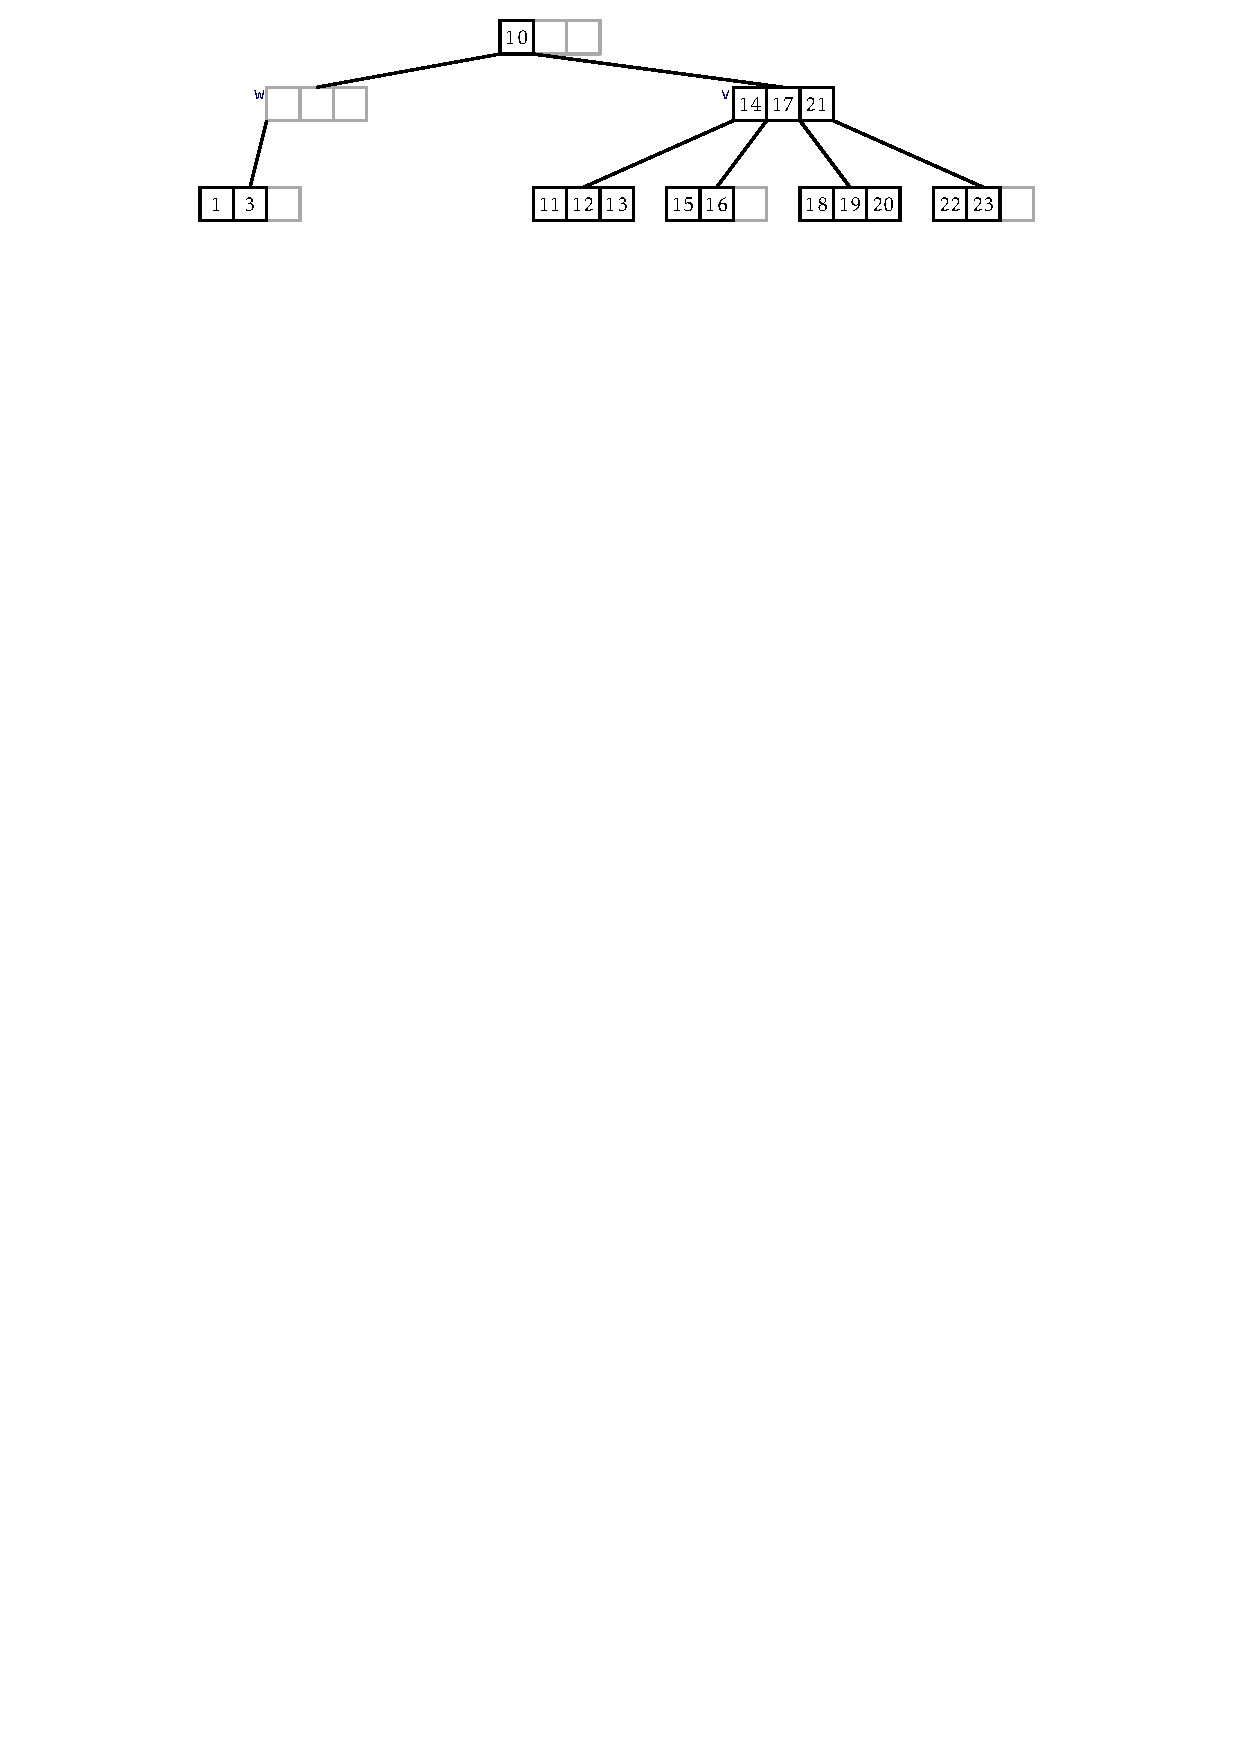
\includegraphics[width=\ScaleIfNeeded]{figs/btree-remove-full-3} \\[2ex]
     \multicolumn{1}{c}{#shiftLR(w,v)#} \\
     \multicolumn{1}{c}{$\Downarrow$} \\[2ex]
     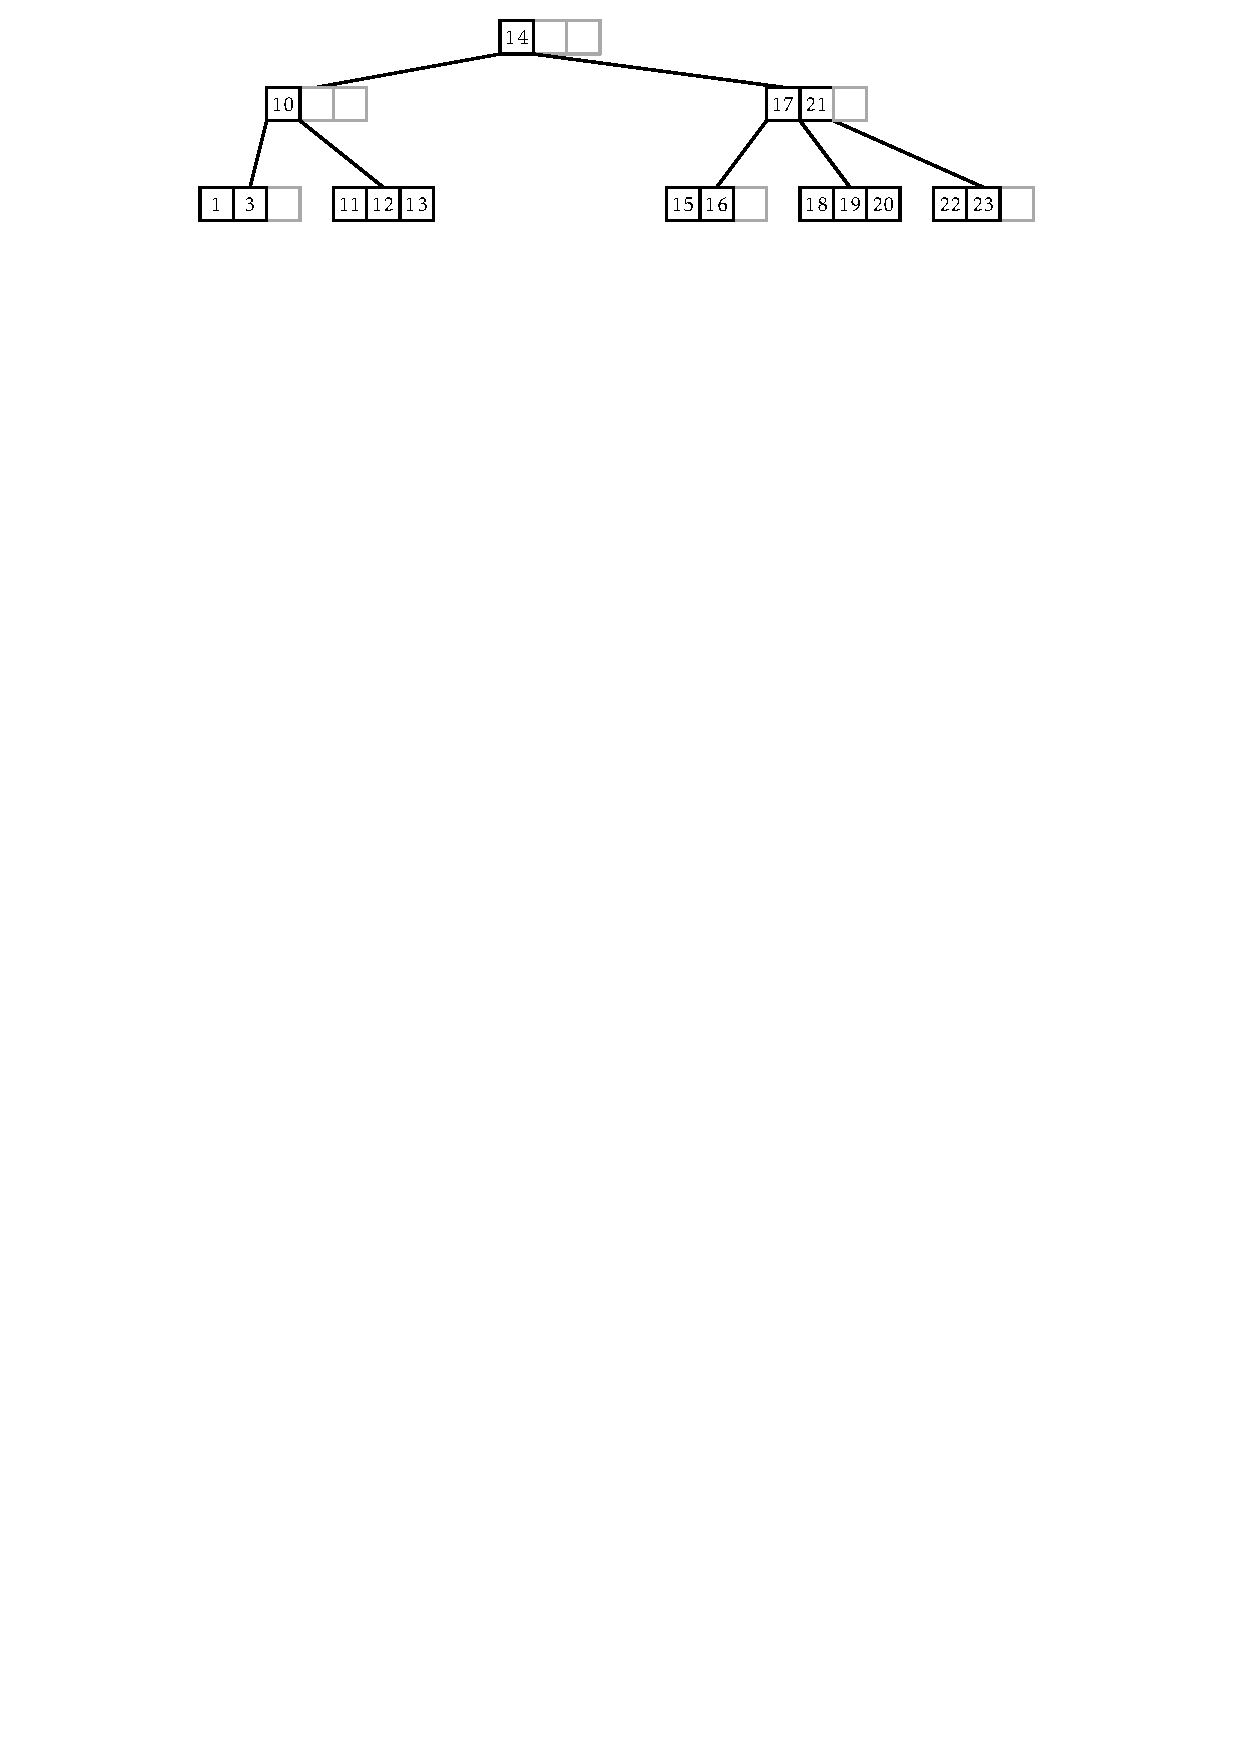
\includegraphics[width=\ScaleIfNeeded]{figs/btree-remove-full-4} \\[2ex]
   \end{tabular}}
   \caption[Removing from a $B$-tree]{Removing the value 4 from a $B$-tree
     results in one merge and one borrowing operation.}
   \figlabel{btree-remove-full}
\end{figure}

When an underflow occurs, #u# either borrows keys from, or is merged with,
one of its siblings.  If #u# is merged with a sibling, then #u#'s parent
will now have one less child and one less key, which can cause #u#'s
parent to underflow; this is again corrected by borrowing or merging,
but merging may cause #u#'s grandparent to underflow.  This process
works its way back up to the root until there is no more underflow or
until the root has its last two children merged into a single child.
When the latter case occurs, the root is removed and its lone child
becomes the new root.

Next we delve into the details of how each of these steps is implemented.
The first job of the #remove(x)# method is to find the element #x# that
should be removed.  If #x# is found in a leaf, then #x# is removed from
this leaf.  Otherwise, if #x# is found at #u.keys[i]# for some internal
node, #u#, then the algorithm removes the smallest value, #x'#, in the
subtree rooted at #u.children[i+1]#.  The value #x'# is the smallest
value stored in the #BTree# that is greater than #x#.  The value of #x'#
is then used to replace #x# in #u.keys[i]#.  This process is illustrated
in \figref{btree-remove}.

\begin{figure}
   \centering{\begin{tabular}{@{}l@{}}
     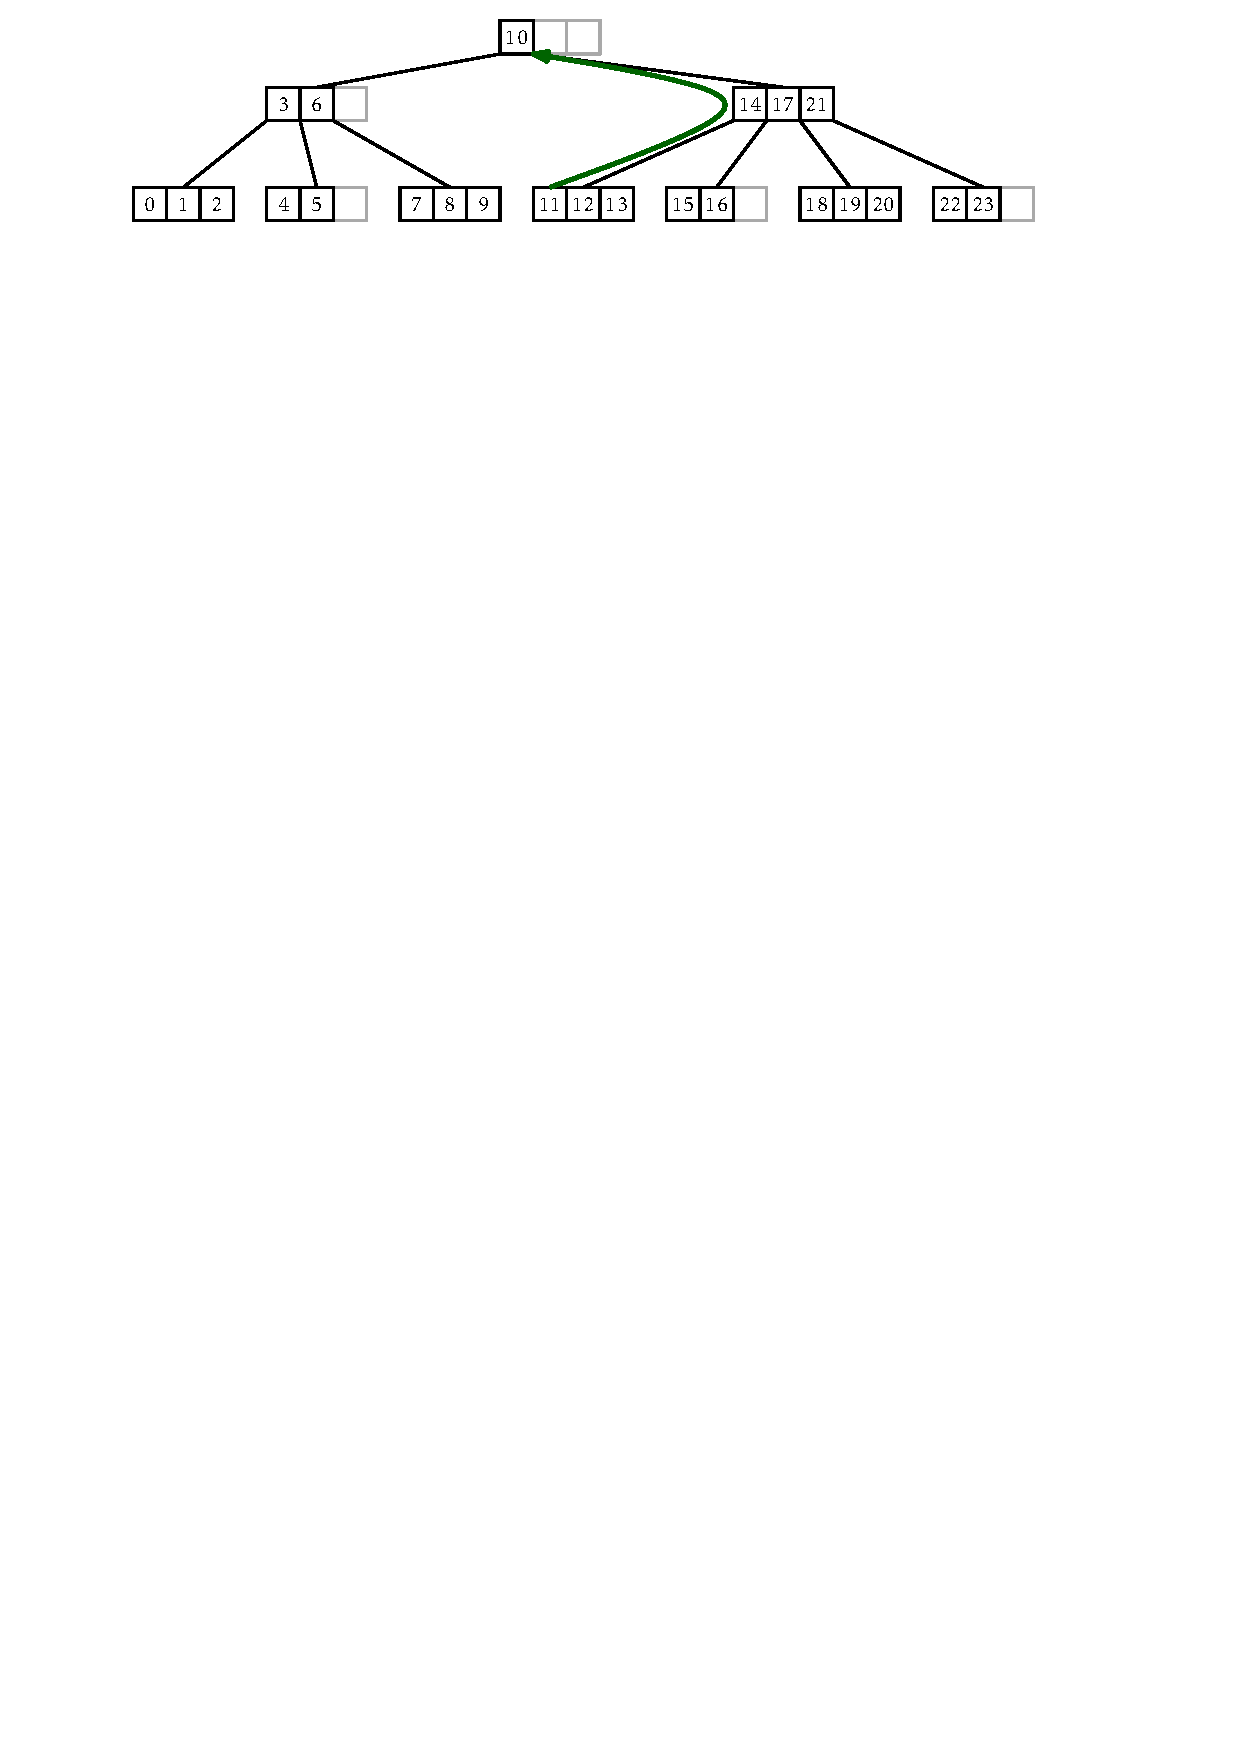
\includegraphics[width=\ScaleIfNeeded]{figs/btree-remove-1} \\[2ex]
     \multicolumn{1}{c}{$\Downarrow$} \\[2ex]
     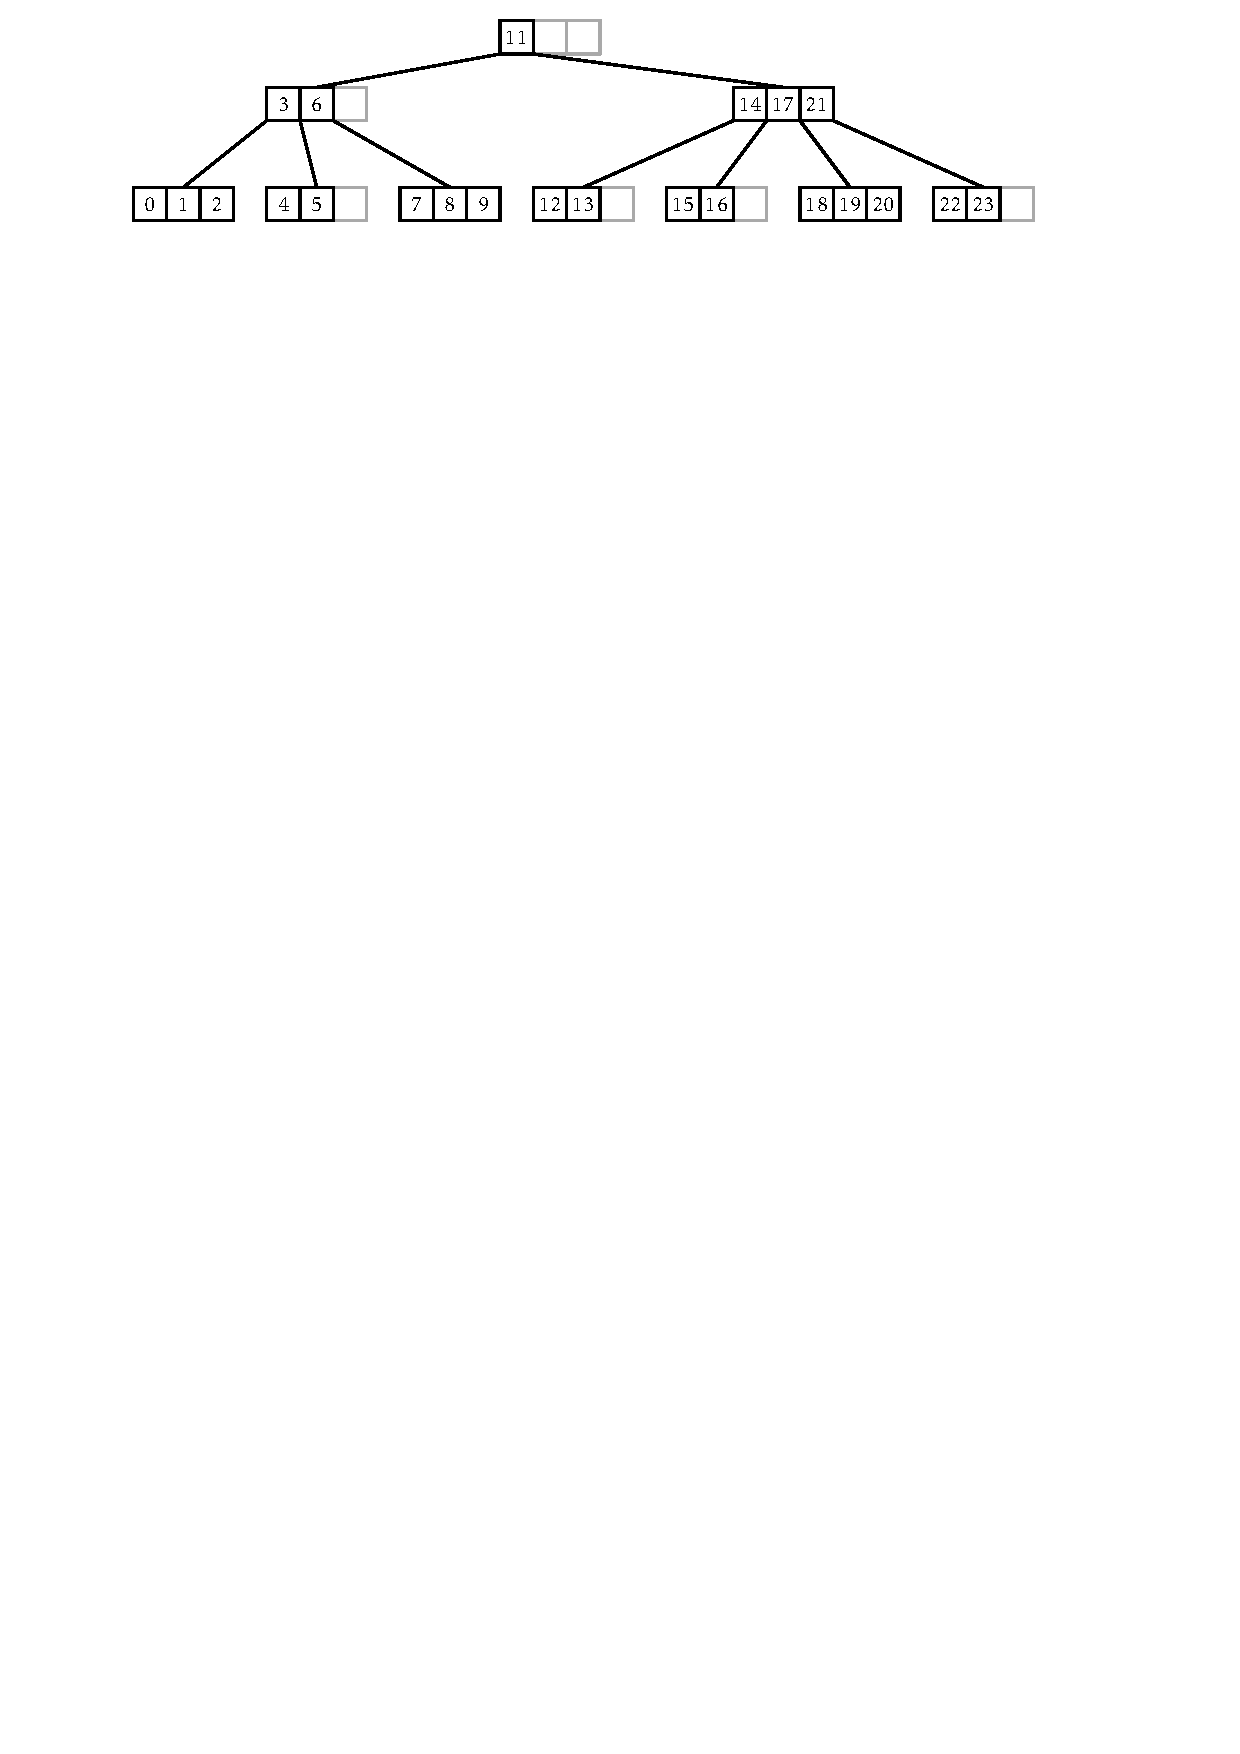
\includegraphics[width=\ScaleIfNeeded]{figs/btree-remove-2} 
   \end{tabular}}
   \caption[The remove operation in a $B$-tree] {The #remove(x)# operation
      in a #BTree#. To remove the value $#x#=10$ we replace it with the
      the value $#x'#=11$ and remove 11 from the leaf that contains it.}
   \figlabel{btree-remove}
\end{figure}

The #removeRecursive(x,ui)# method is a recursive implementation of the
preceding algorithm:
\codeimport{ods/BTree.removeRecursive(x,ui).removeSmallest(ui)}

Note that, after recursively removing the value #x# from the #i#th child of #u#,
#removeRecursive(x,ui)# needs to ensure that this child still has at
least $B-1$ keys.  In the preceding code, this is done using a
method called #checkUnderflow(x,i)#, which checks for and corrects an
underflow in the #i#th child of #u#.  Let #w# be the #i#th child of #u#.
If #w# has only $B-2$ keys, then this needs to be fixed.  The fix
requires using a sibling of #w#.  This can be either child $#i#+1$ of
#u# or child $#i#-1$ of #u#.  We will usually use child $#i#-1$ of #u#,
which is the sibling, #v#, of #w# directly to its left.  The only time
this doesn't work is when $#i#=0$, in which case we use the sibling
directly to #w#'s right.
\codeimport{ods/BTree.checkUnderflow(u,i)}
In the following, we focus on the case when $#i#\neq 0$ so that any
underflow at the #i#th child of #u# will be corrected with the help
of the $(#i#-1)$st child of #u#.  The case $#i#=0$ is similar and the
details can be found in the accompanying source code.

To fix an underflow at node #w#, we need to find more keys (and possibly
also children), for #w#.  There are two ways to do this:

\begin{description}
  \item[Borrowing:]
  \index{borrow}%
  If #w# has a sibling, #v#, with more than $B-1$ keys,
  then #w# can borrow some keys (and possibly also children) from #v#.
  More specifically, if #v# stores #size(v)# keys, then between them,
  #v# and #w# have a total of
  \[
     B-2 + #size(w)# \ge 2B-2
  \]
  keys.  We can therefore shift keys from #v# to #w# so that each of
  #v# and #w# has at least $B-1$ keys.  This process is illustrated in
  \figref{btree-borrow}.

  \begin{figure}
      \centering{\begin{tabular}{@{}l@{}}
       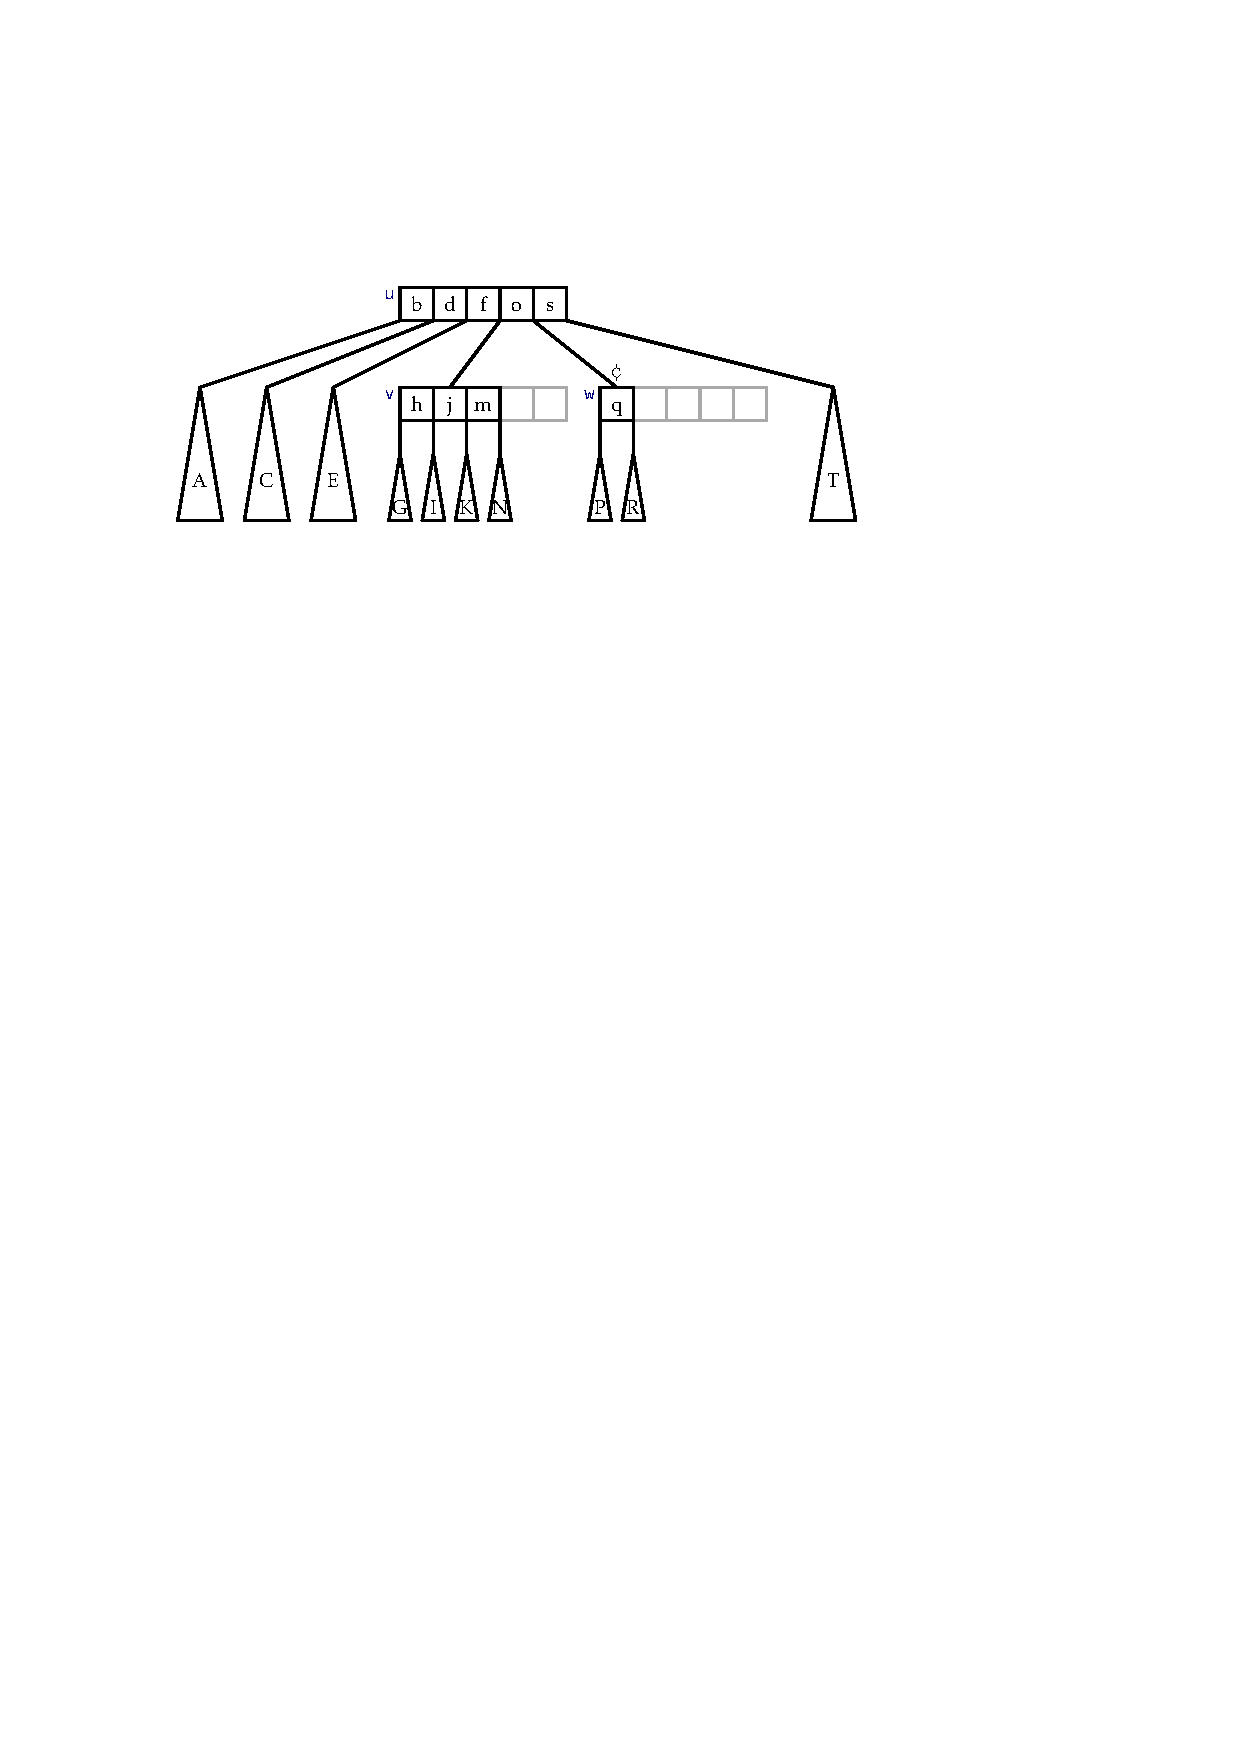
\includegraphics[width=\ScaleIfNeeded]{figs/btree-borrow-1} \\[2ex]
       \multicolumn{1}{c}{#shiftRL(v,w)#} \\ 
       \multicolumn{1}{c}{$\Downarrow$} \\[2ex]
       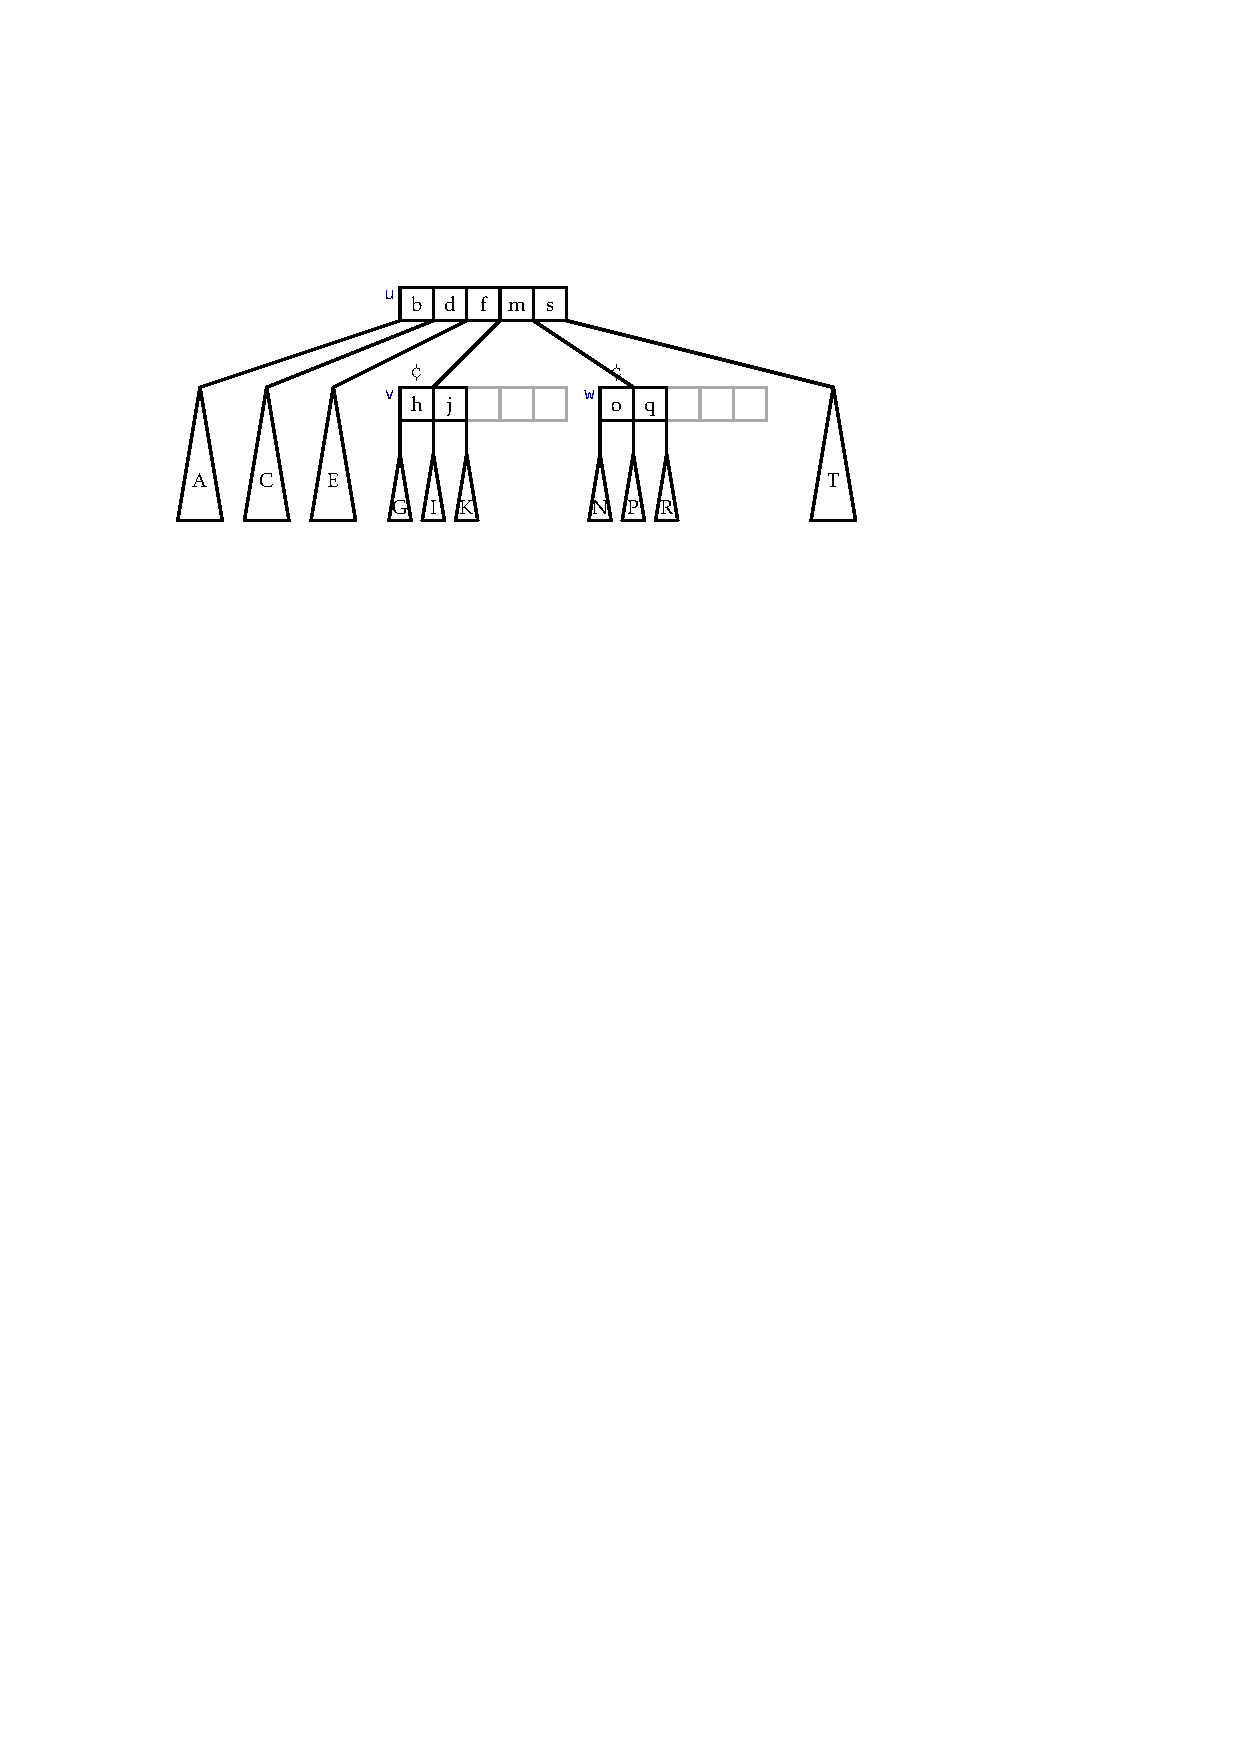
\includegraphics[width=\ScaleIfNeeded]{figs/btree-borrow-2} \\
     \end{tabular}}
    \caption[Borrowing in a $B$-tree]{If #v# has more than $B-1$ keys,
       then #w# can borrow keys from #v#.}
    \figlabel{btree-borrow}
  \end{figure}
  
  \item[Merging:]
  \index{merge}%
  If #v# has only $B-1$ keys, we must do something more
  drastic, since #v# cannot afford to give any keys to #w#.  Therefore,
  we \emph{merge} #v# and #w# as shown in \figref{btree-merge}.  The merge
  operation is the opposite of the split operation.  It takes two nodes
  that contain a total of $2B-3$ keys and merges them into a single
  node that contains $2B-2$ keys.  (The additional key comes from the
  fact that, when we merge #v# and #w#, their common parent, #u#, now
  has one less child and therefore needs to give up one of its keys.)
  
  \begin{figure}
     \centering{\begin{tabular}{@{}l@{}}
       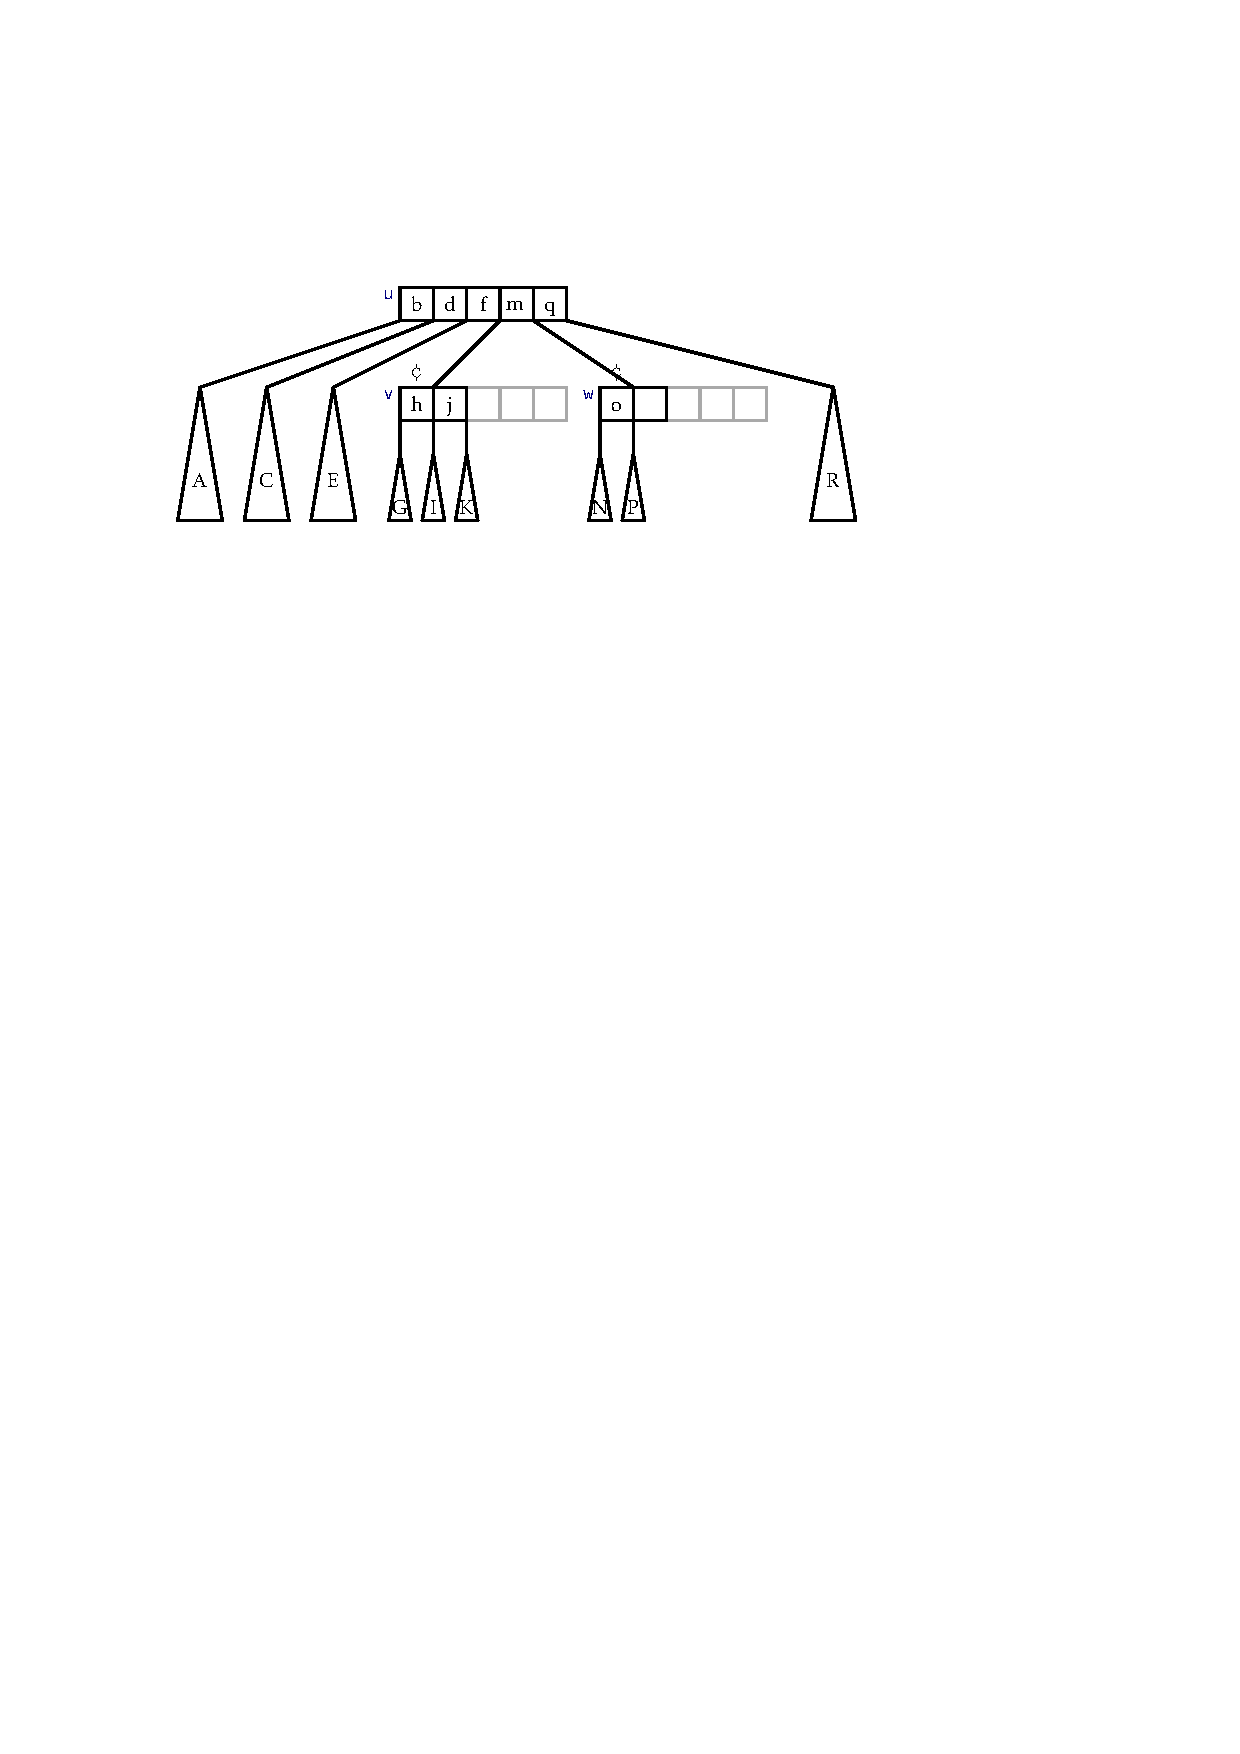
\includegraphics[width=\ScaleIfNeeded]{figs/btree-merge-1} \\[2ex]
       \multicolumn{1}{c}{#merge(v,w)#} \\ 
       \multicolumn{1}{c}{$\Downarrow$} \\[2ex]
       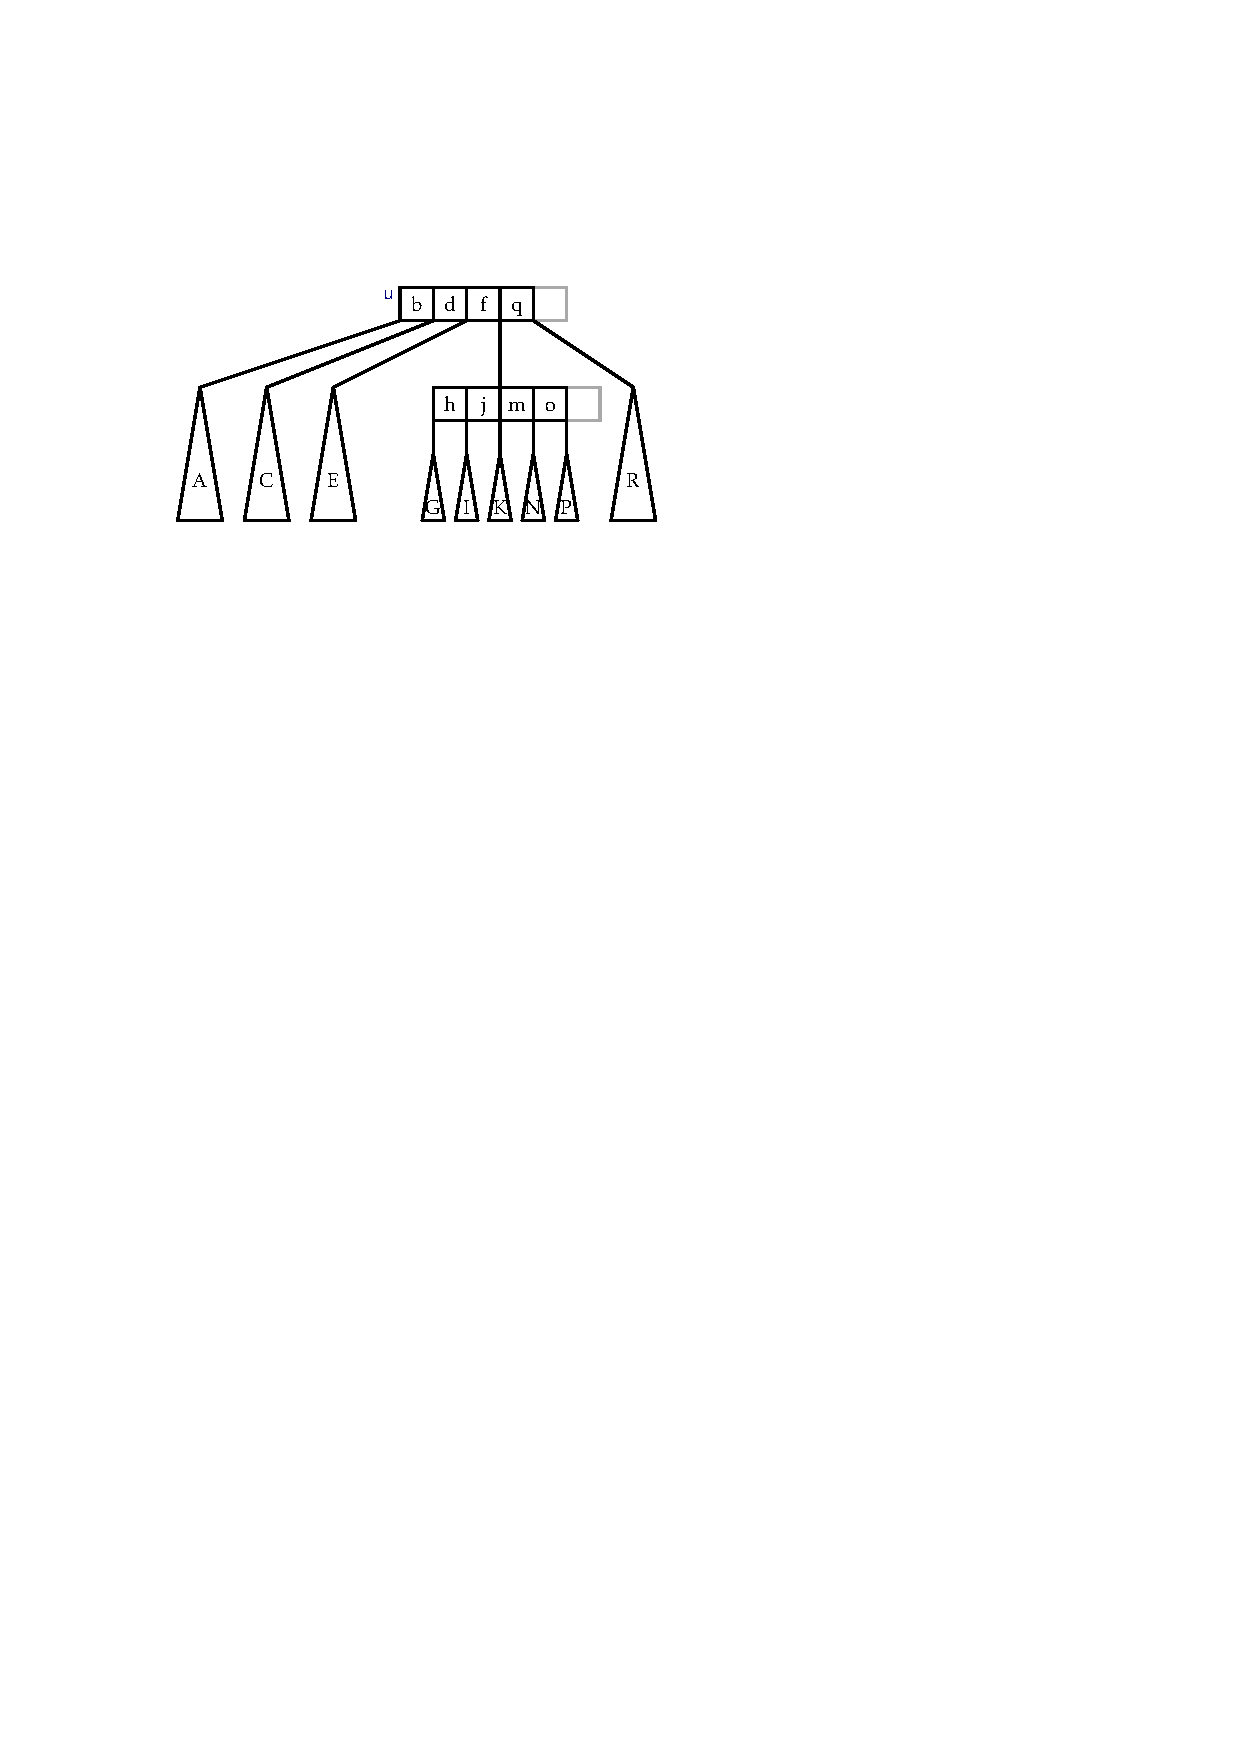
\includegraphics[width=\ScaleIfNeeded]{figs/btree-merge-2} \\
     \end{tabular}}
     \caption[Merging in a $B$-tree]{Merging two siblings #v# and #w#
     in a $B$-tree ($B=3$).}
     \figlabel{btree-merge}
  \end{figure}
\end{description}

\codeimport{ods/BTree.checkUnderflowNonZero(u,i).checkUnderflowZero(u,i)}

To summarize, the #remove(x)# method in a $B$-tree follows a root to
leaf path, removes a key #x'# from a leaf, #u#, and then performs zero
or more merge operations involving #u# and its ancestors, and performs
at most one borrowing operation.  Since each merge and borrow operation
involves modifying only three nodes, and only $O(\log_B #n#)$ of these
operations occur, the entire process takes $O(\log_B #n#)$ time in the
external memory model.  Again, however, each merge and borrow operation
takes $O(B)$ time in the word-RAM model, so (for now) the most we can
say about the running time required by #remove(x)# in the word-RAM model
is that it is $O(B\log_B #n#)$.

\subsection{Amortized Analysis of $B$-Trees}
\seclabel{btree-amortized}

Thus far, we have shown that
\begin{enumerate}
  \item In the external memory model, the running time of #find(x)#,
    #add(x)#, and #remove(x)# in a $B$-tree is $O(\log_B #n#)$.
  \item In the word-RAM model, the running time of #find(x)# is $O(\log #n#)$
    and the running time of #add(x)# and #remove(x)# is $O(B\log #n#)$.
\end{enumerate}

The following lemma shows that, so far, we have overestimated the number of merge and split operations performed by $B$-trees.

\begin{lem}\lemlabel{btree-split}
  Starting with an empty $B$-tree and performing any sequence of
  $m$ #add(x)# and #remove(x)# operations results in at most $3m/2$ splits,
  merges, and borrows being performed.
\end{lem}

\begin{proof}
   The proof of this has already been sketched in
   \secref{redblack-summary} for the special case in which $B=2$.
   The lemma can be proven using a credit scheme,
   \index{credit scheme}%
   in which
  \begin{enumerate}
    \item each split, merge, or borrow operation is paid for with two
      credits, i.e., a credit is removed each time one of these operations
      occurs; and
    \item at most three credits are created during any #add(x)# or
      #remove(x)# operation.
  \end{enumerate}
  Since at most $3m$ credits are ever created and each split,
  merge, and borrow is paid for with with two credits, it follows
  that at most $3m/2$ splits, merges, and borrows are performed.
  These credits are illustrated using the \cent\ symbol in
  Figures~\ref{fig:btree-split}, \ref{fig:btree-borrow}, and
  \ref{fig:btree-merge}.

  To keep track of these credits the proof maintains the following
  \emph{credit invariant}:
  \index{credit invariant}%
  Any non-root node with $B-1$ keys stores one
  credit and any node with $2B-1$ keys stores three credits.  A node
  that stores at least $B$ keys and most $2B-2$ keys need not store
  any credits.  What remains is to show that we can maintain the credit
  invariant and satisfy properties 1 and 2, above, during each #add(x)#
  and #remove(x)# operation.

  \paragraph{Adding:}
  The #add(x)# method does not perform any merges or borrows, so we
  need only consider split operations that occur as a result of calls
  to #add(x)#.

  Each split operation occurs because a key is added to a node, #u#, that
  already contains $2B-1$ keys.  When this happens, #u# is split into two
  nodes, #u'# and #u''# having $B-1$ and $B$ keys, respectively.  Prior to
  this operation, #u# was storing $2B-1$ keys, and hence three credits.
  Two of these credits can be used to pay for the split and the other
  credit can be given to #u'# (which has $B-1$ keys) to maintain the
  credit invariant.  Therefore, we can pay for the split and maintain
  the credit invariant during any split.

  The only other modification to nodes that occur during an #add(x)#
  operation happens after all splits, if any, are complete.  This
  modification involves adding a new key to some node #u'#.  If, prior
  to this, #u'# had $2B-2$ children, then it now has $2B-1$ children and
  must therefore receive three credits.  These are the only credits given
  out by the #add(x)# method.

  \paragraph{Removing:}
  During a call to #remove(x)#, zero or more merges occur and are possibly
  followed by a single borrow.  Each merge occurs because two nodes,
  #v# and #w#, each of which had exactly $B-1$ keys prior to calling
  #remove(x)# were merged into a single node with exactly $2B-2$ keys.
  Each such merge therefore frees up two credits that can be used to
  pay for the merge.

  After any merges are performed, at most one borrow operation occurs,
  after which no further merges or borrows occur.  This borrow operation
  only occurs if we remove a key from a leaf, #v#, that has $B-1$ keys.
  The node #v# therefore has one credit, and this credit goes towards
  the cost of the borrow.  This single credit is not enough to pay for
  the borrow, so we create one credit to complete the payment.

  At this point, we have created one credit and we still need to show
  that the credit invariant can be maintained.  In the worst case,
  #v#'s sibling, #w#, has exactly $B$ keys before the borrow so that,
  afterwards, both #v# and #w# have $B-1$ keys.  This means that #v# and
  #w# each should be storing a credit when the operation is complete.
  Therefore, in this case, we create an additional two credits to give to
  #v# and #w#.  Since a borrow happens at most once during a #remove(x)#
  operation, this means that we create at most three credits, as required.

  If the #remove(x)# operation does not include a borrow operation, this
  is because it finishes by removing a key from some node that, prior
  to the operation, had $B$ or more keys.  In the worst case, this node
  had exactly $B$ keys, so that it now has $B-1$ keys and must be given
  one credit, which we create.

  In either case---whether the removal finishes with a borrow
  operation or not---at most three credits need to be created during a
  call to #remove(x)# to maintain the credit invariant and pay for all
  borrows and merges that occur. This completes the proof of the lemma.
\end{proof}

The purpose of \lemref{btree-split} is to show that, in the word-RAM
model the cost of splits, merges and joins during a sequence of $m$
#add(x)# and #remove(x)# operations is only $O(Bm)$.  That is, the
amortized cost per operation is only $O(B)$, so the amortized cost
of #add(x)# and #remove(x)# in the word-RAM model is $O(B+\log #n#)$.
This is summarized by the following pair of theorems:

\begin{thm}[External Memory $B$-Trees]
  A #BTree# implements the #SSet# interface. In the external memory model,
  a #BTree# supports the operations #add(x)#, #remove(x)#, and #find(x)#
  in $O(\log_B #n#)$ time per operation.
\end{thm}

\begin{thm}[Word-RAM $B$-Trees]
  A #BTree# implements the #SSet# interface. In the word-RAM model, and
  ignoring the cost of splits, merges, and borrows, a #BTree# supports
  the operations #add(x)#, #remove(x)#, and #find(x)# in $O(\log #n#)$
  time per operation.
  Furthermore, beginning with an empty #BTree#, any sequence of $m$
  #add(x)# and #remove(x)# operations results in a total of $O(Bm)$
  time spent performing splits, merges, and borrows.
\end{thm}

\section{Discussion and Exercises}

The external memory model of computation was introduced by Aggarwal and
Vitter \cite{av88}.  It is sometimes also called the \emph{I/O model}
\index{I/O model}%
or the \emph{disk access model}. 
\index{disk access model}%

$B$-Trees are to external memory searching what binary search trees
are to internal memory searching.  $B$-trees were introduced by Bayer
and McCreight \cite{bm70} in 1970 and, less than ten years later, the
title of Comer's ACM Computing Surveys article referred to
them as ubiquitous \cite{c79}.

Like binary search trees, there are many variants of $B$-Trees, including
$B^+$-trees,
\index{B+-tree@$B^+$-tree}%
$B^*$-trees,
\index{B*-tree@$B^*$-tree}%
and counted $B$-trees.
\index{conted $B$-tree}%
$B$-trees are indeed
ubiquitous and are the primary data structure in many file systems,
including Apple's HFS+,
\index{HFS+}%
Microsoft's NTFS, 
\index{NTFS}%
and Linux's Ext4;
\index{Ext4}%
every
major database system; and key-value stores used in cloud computing.
Graefe's recent survey \cite{g10} provides a 200+ page overview of the
many modern applications, variants, and optimizations of $B$-trees.

$B$-trees implement the #SSet# interface.  If only the #USet# interface
is needed, then external memory hashing
\index{external memory hashing}%
could be used as an alternative
to $B$-trees.  External memory hashing schemes do exist; see, for example,
Jensen and Pagh~\cite{jp08}.  These schemes implement the #USet# operations
in $O(1)$ expected time in the external memory model. However, for a
variety of reasons, many applications still use $B$-trees even though
they only require #USet# operations.

One reason $B$-trees are such a popular choice is that they often perform
better than their $O(\log_B #n#)$ running time bounds suggest. The
reason for this is that, in external memory settings, the value of $B$
is typically quite large---in the hundreds or even thousands.  This means
that 99\% or even 99.9\% of the data in a $B$-tree is stored in the
leaves.  In a database system with a large memory, it may be possible
to cache all the internal nodes of a $B$-tree in RAM, since they only
represent 1\% or 0.1\% of the total data set.  When this happens,
this means that a search in a $B$-tree involves a very fast search in
RAM, through the internal nodes, followed by a single external memory
access to retrieve a leaf.

\begin{exc}
  Show what happens when the keys 1.5 and then 7.5 are added to the
  $B$-tree in \figref{btree}.
\end{exc}

\begin{exc}
  Show what happens when the keys 3 and then 4 are removed from the
  $B$-tree in \figref{btree}.
\end{exc}

\begin{exc}
  What is the maximum number of internal nodes in a $B$-tree that stores
  #n# keys (as a function of #n# and $B$)?
\end{exc}

\begin{exc}
  The introduction to this chapter claims that $B$-trees only need an
  internal memory of size $O(B+\log_B#n#)$.  However, the implementation
  given here actually requires more memory.
  \begin{enumerate}
    \item Show that the implementation of the #add(x)# and #remove(x)#
      methods given in this chapter use an internal memory
      proportional to $B\log_B #n#$.
    \item Describe how these methods could be modified in order to reduce their memory
      consumption to $O(B + \log_B #n#)$.
  \end{enumerate}
\end{exc}

\begin{exc}
  Draw the credits used in the proof of \lemref{btree-split} on the trees
  in Figures~\ref{fig:btree-add} and \ref{fig:btree-remove-full}.  Verify
  that (with three additional credits) it is possible to pay for the splits, 
  merges, and borrows and maintain the credit invariant.
\end{exc}

\begin{exc}
  Design a modified version of a $B$-tree in which nodes can have anywhere
  from $B$ up to $3B$ children (and hence $B-1$ up to $3B-1$ keys).
  Show that this new version of $B$-trees performs only $O(m/B)$ splits,
  merges, and borrows during a sequence of $m$ operations.  (Hint:
  For this to work, you will have to be more agressive with merging,
  sometimes merging two nodes before it is strictly necessary.)
\end{exc}

\begin{exc}
  In this exercise, you will design a modified method of splitting and
  merging in $B$-trees that asymptotically reduces the number of splits,
  borrows and merges by considering up to three nodes at a time.
  \begin{enumerate}
    \item Let #u# be an overfull node and let #v# be a sibling immediately
    to the right of #u#.  There are two ways to fix the overflow at #u#:
    \begin{enumerate}
       \item #u# can give some of its keys to #v#; or
       \item #u# can be split and the keys of #u# and #v# can be evenly
        distributed among #u#, #v#, and the newly created node, #w#.
    \end{enumerate}
    Show that this can always be done in such a way that, after the
    operation, each of the (at most 3) affected nodes has at least
    $B+\alpha B$ keys and at most $2B-\alpha B$ keys, for some constant
    $\alpha > 0$.
    \item Let #u# be an underfull node and let #v# and #w# be siblings of #u#
    There are two ways to fix the underflow at #u#:
    \begin{enumerate}
       \item keys can be redistributed among #u#, #v#, and #w#; or
       \item #u#, #v#, and #w# can be merged into two nodes and the keys
        of #u#, #v#, and #w# can be redistributed amongst these nodes.
    \end{enumerate}
    Show that this can always be done in such a way that, after the
    operation, each of the (at most 3) affected nodes has at least
    $B+\alpha B$ keys and at most $2B-\alpha B$ keys, for some constant
    $\alpha > 0$.
    \item Show that, with these modifications, the number of 
      merges, borrows, and splits that occur during $m$ operations is $O(m/B)$.
  \end{enumerate}
\end{exc}


\begin{exc}
  A $B^+$-tree, illustrated in \figref{bplustree} stores every key in a
  leaf and keeps its leaves stored as a doubly-linked list.  As usual,
  each leaf stores between $B-1$ and $2B-1$ keys.  Above this list is
  a standard $B$-tree that stores the largest value from each leaf but
  the last.
  \begin{enumerate}
    \item Describe fast implementations of #add(x)#, #remove(x)#,
      and #find(x)# in a $B^+$-tree.
    \item Explain how to efficiently implement the #findRange(x,y)# method,
      that reports all values
      greater than #x# and less than or equal to #y#, in
      a $B^+$-tree.
    \item Implement a class, #BPlusTree#, that implements #find(x)#,
      #add(x)#, #remove(x)#, and #findRange(x,y)#.
      \index{BPlusTree@#BPlusTree#}%
    \item $B^+$-trees duplicate some of the keys because they are stored
      both in the $B$-tree and in the list.  Explain why this duplication
      does not add up to much for large values of $B$.
  \end{enumerate}
\end{exc}

\begin{figure}
  \centering{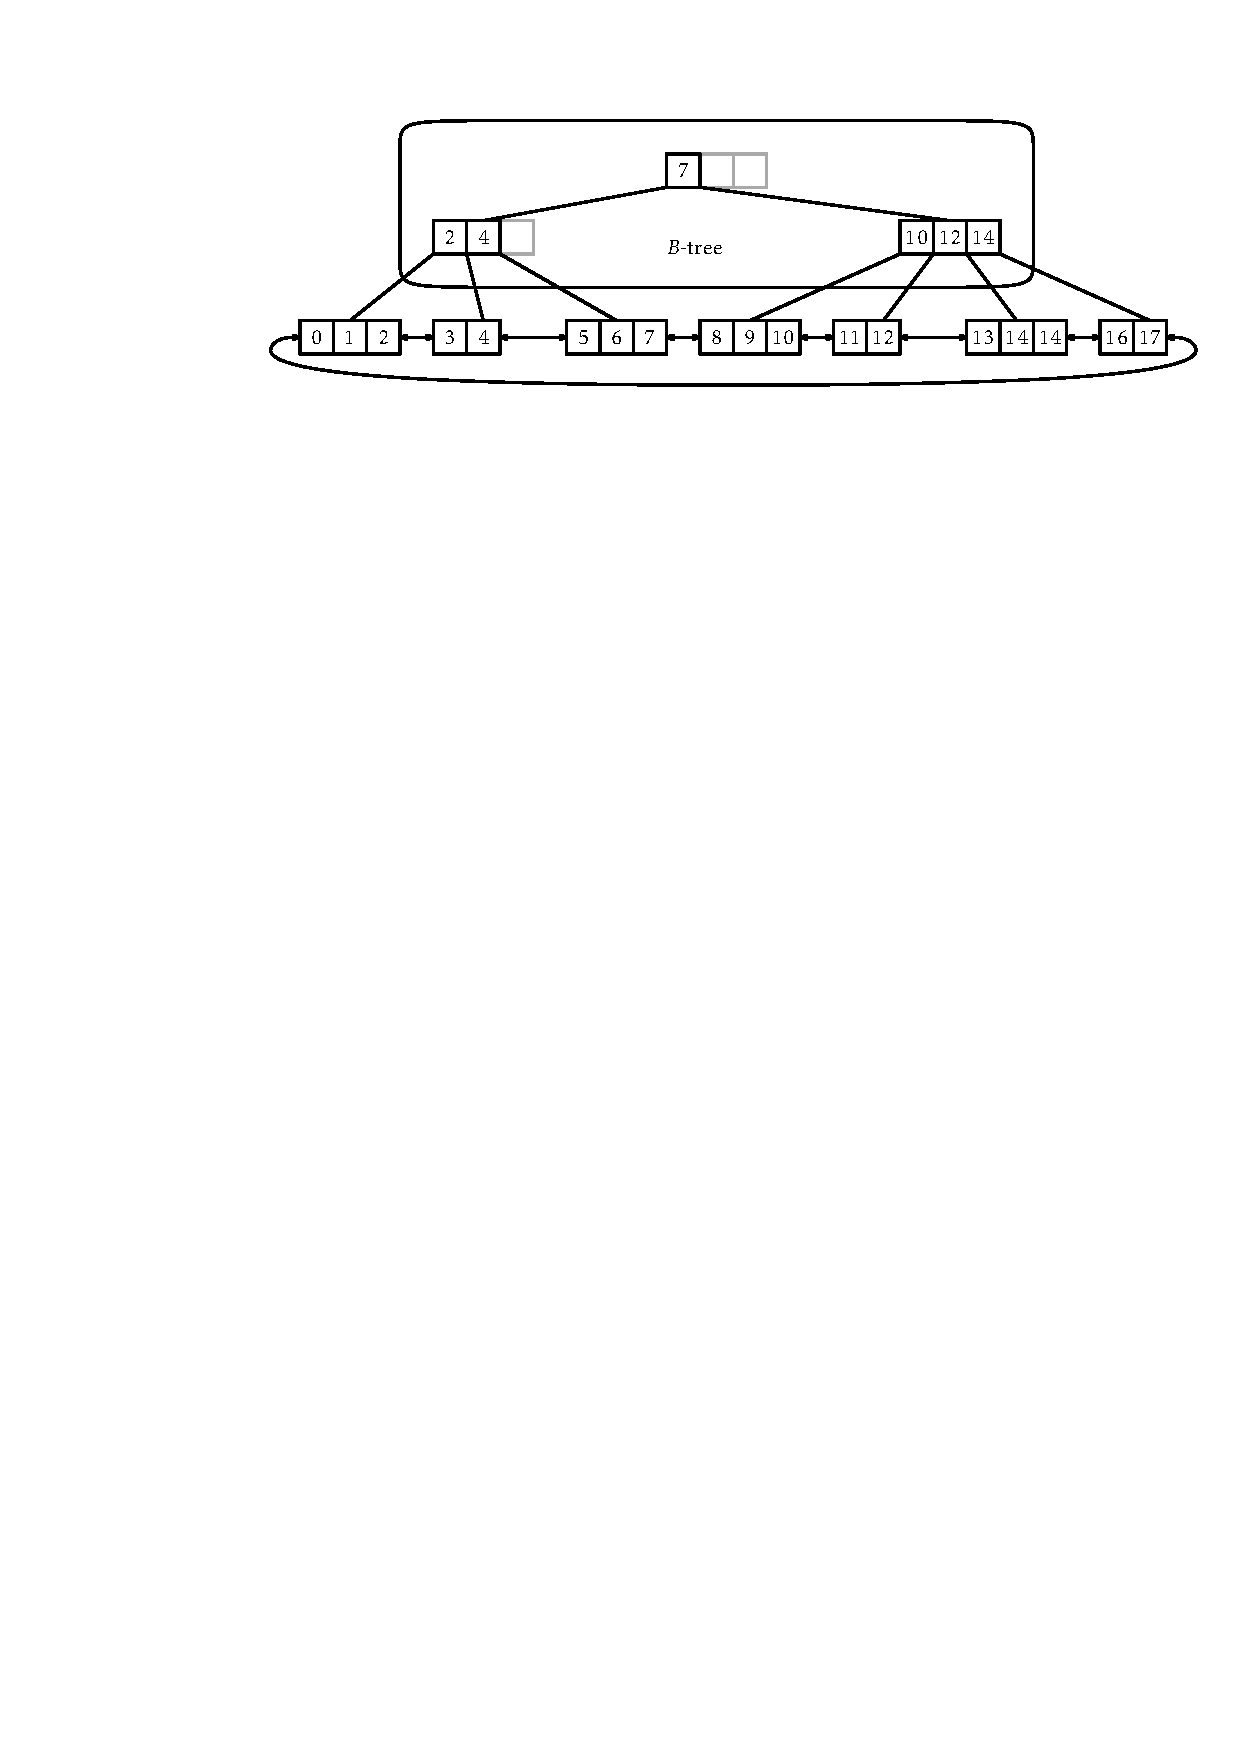
\includegraphics[width=\ScaleIfNeeded]{figs/bplustree}} 
  \caption{A $B^+$-tree is a $B$-tree on top of a doubly-linked list of blocks.}
  \figlabel{bplustree}
\end{figure}


